\documentclass[11pt,xcolor=dvipsnames,professionalfonts,notes]{beamer}

% Pakete
\usepackage[utf8]{inputenc}
\usepackage[english]{babel}

% AMS Pakete
\usepackage{amsmath}
\usepackage{amsfonts}
\usepackage{amssymb}
\usepackage{mathtools}

% Text tools
\usepackage{textcomp}

% Einheiten
\usepackage{siunitx}
\sisetup{
	separate-uncertainty
}

% Grafiken
\usepackage{graphicx}
\usepackage{booktabs}
\setbeamerfont{caption}{size=\footnotesize}
\setbeamertemplate{caption}{\raggedright\insertcaption\par}
\usepackage[percent]{overpic}

% Theme
\usetheme{Boadilla}
\usecolortheme{rose}
\useoutertheme{infolines}
\useinnertheme{rectangles}
\setbeamertemplate{itemize subitem}[triangle]

\usefonttheme[onlymath]{serif}

% [num] Zitationen
\setbeamertemplate{bibliography item}[text]

% Navigationsleiste ausschalten
\beamertemplatenavigationsymbolsempty

\author[Christopher Deutsch]
{Christopher Deutsch}

\title
{Interactions of photons with matter}

\subtitle
{}
%\logo{}

\institute[]
{Joint BCGS Seminar on Detectors in Nuclear and Particle Physics\\ Summer Term 16}

\date{2.\ May 2016}

%\setbeamercovered{transparent}
%\setbeamertemplate{navigation symbols}{}

\newcommand{\beginbackup}{
	\newcounter{framenumbervorappendix}
	\setcounter{framenumbervorappendix}{\value{framenumber}}
}
\newcommand{\backupend}{
	\addtocounter{framenumbervorappendix}{-\value{framenumber}}
	\addtocounter{framenumber}{\value{framenumbervorappendix}} 
}

\begin{document}
\maketitle

\begin{frame}{Interactions of photons with matter}
	\tableofcontents
\end{frame}

\note[itemize]{
	\item Photoelectric effect
	
	\item Compton effect
	
	\item Pair production
	
	\item Electromagnetic showers
	
	\item Detector concepts		
}

\section{Introduction}

\subsection{Charged particle interaction}

\begin{frame}{Introduction -- charged particle interactions}
	Interaction of \textbf{charged particles} with matter:
	\begin{itemize}
		\item energy loss due to inelastic collisions with atomic electrons
		\item range $R$
	\end{itemize}
	\vfill
	\begin{center}
		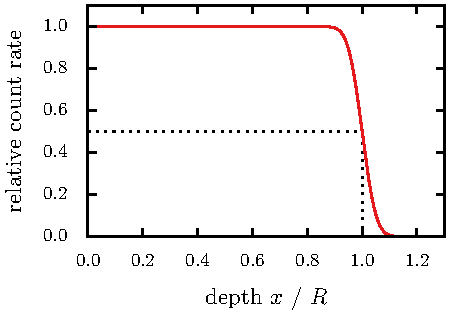
\includegraphics{./figures/range.pdf}
	\end{center}
\end{frame}

\note[itemize]{
	\item charged particles
	\begin{itemize}
		\item fixed range
	\end{itemize}
	
	\item photons
	\begin{itemize}
		\item uncharged
	\end{itemize}
}


\subsection{Photon interaction}

\begin{frame}{Introduction -- photon interactions}
	\begin{columns}
		\column[c]{0.4\textwidth}
			\begin{center}
				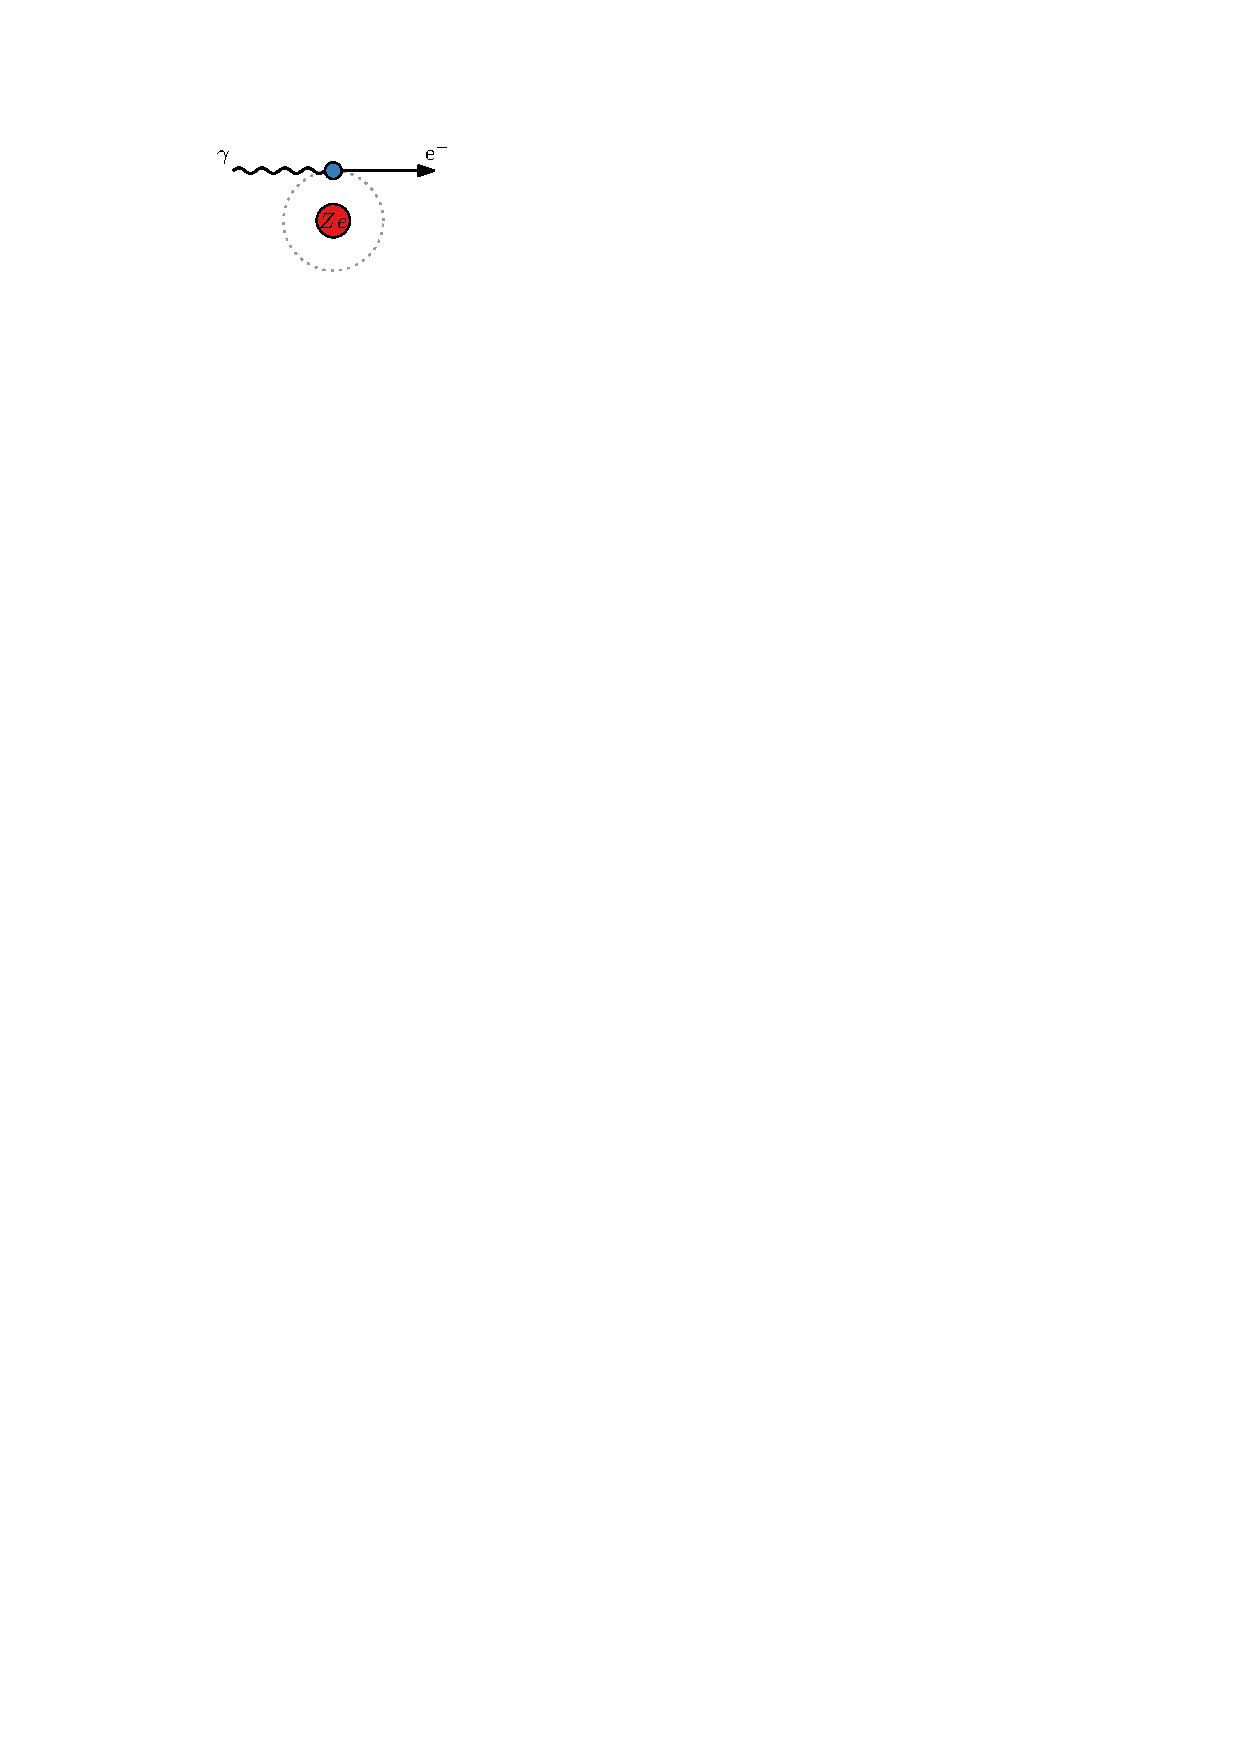
\includegraphics{./figures/photoeffect_intro.pdf}
			\end{center}
		
		\column[c]{0.6\textwidth}
			Photoelectric effect
	\end{columns}
	\vspace{-0.2cm}
	\begin{columns}
		\column[c]{0.4\textwidth}
		\begin{center}
			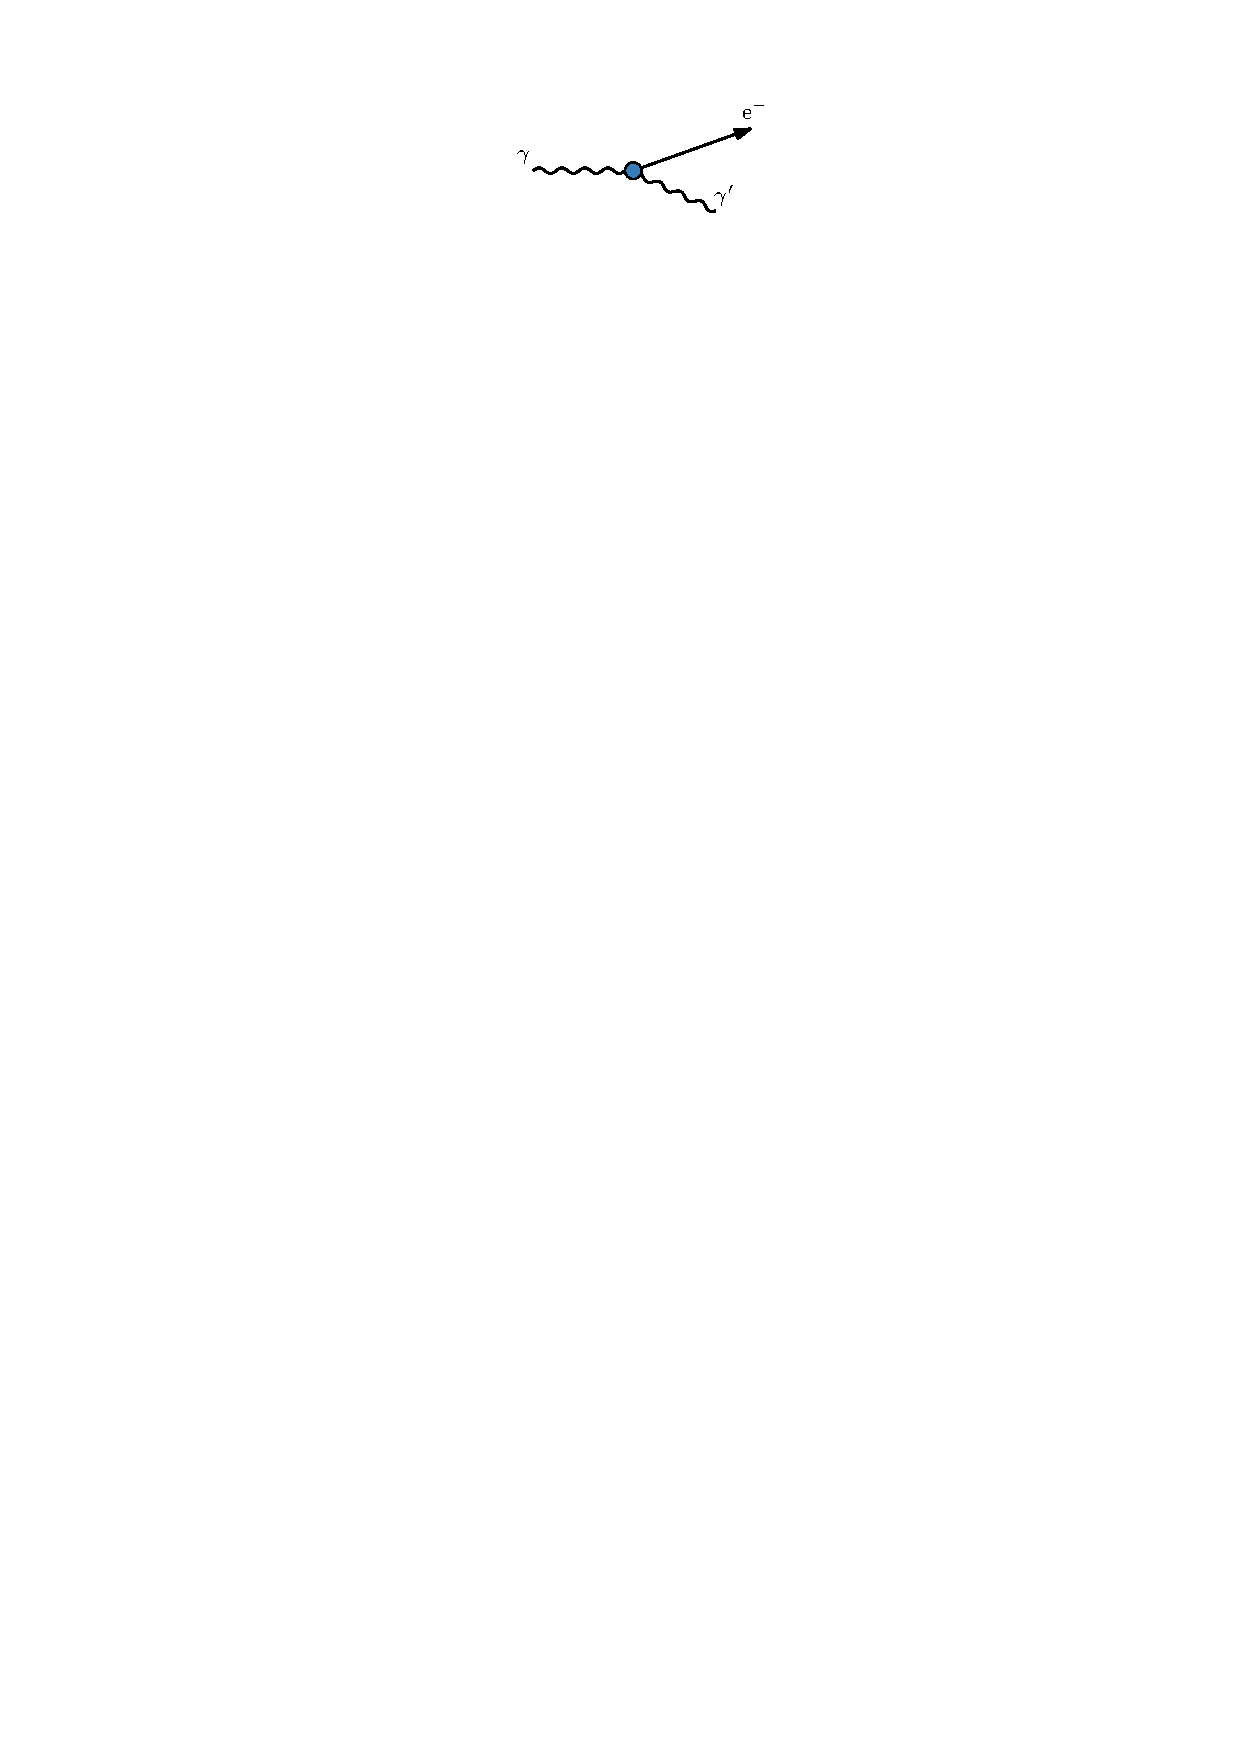
\includegraphics{./figures/compton_intro.pdf}
		\end{center}
		
		\column[c]{0.6\textwidth}
		Compton effect
	\end{columns}
	\vspace{0.2cm}
	\begin{columns}
		\column[c]{0.4\textwidth}
		\begin{center}
			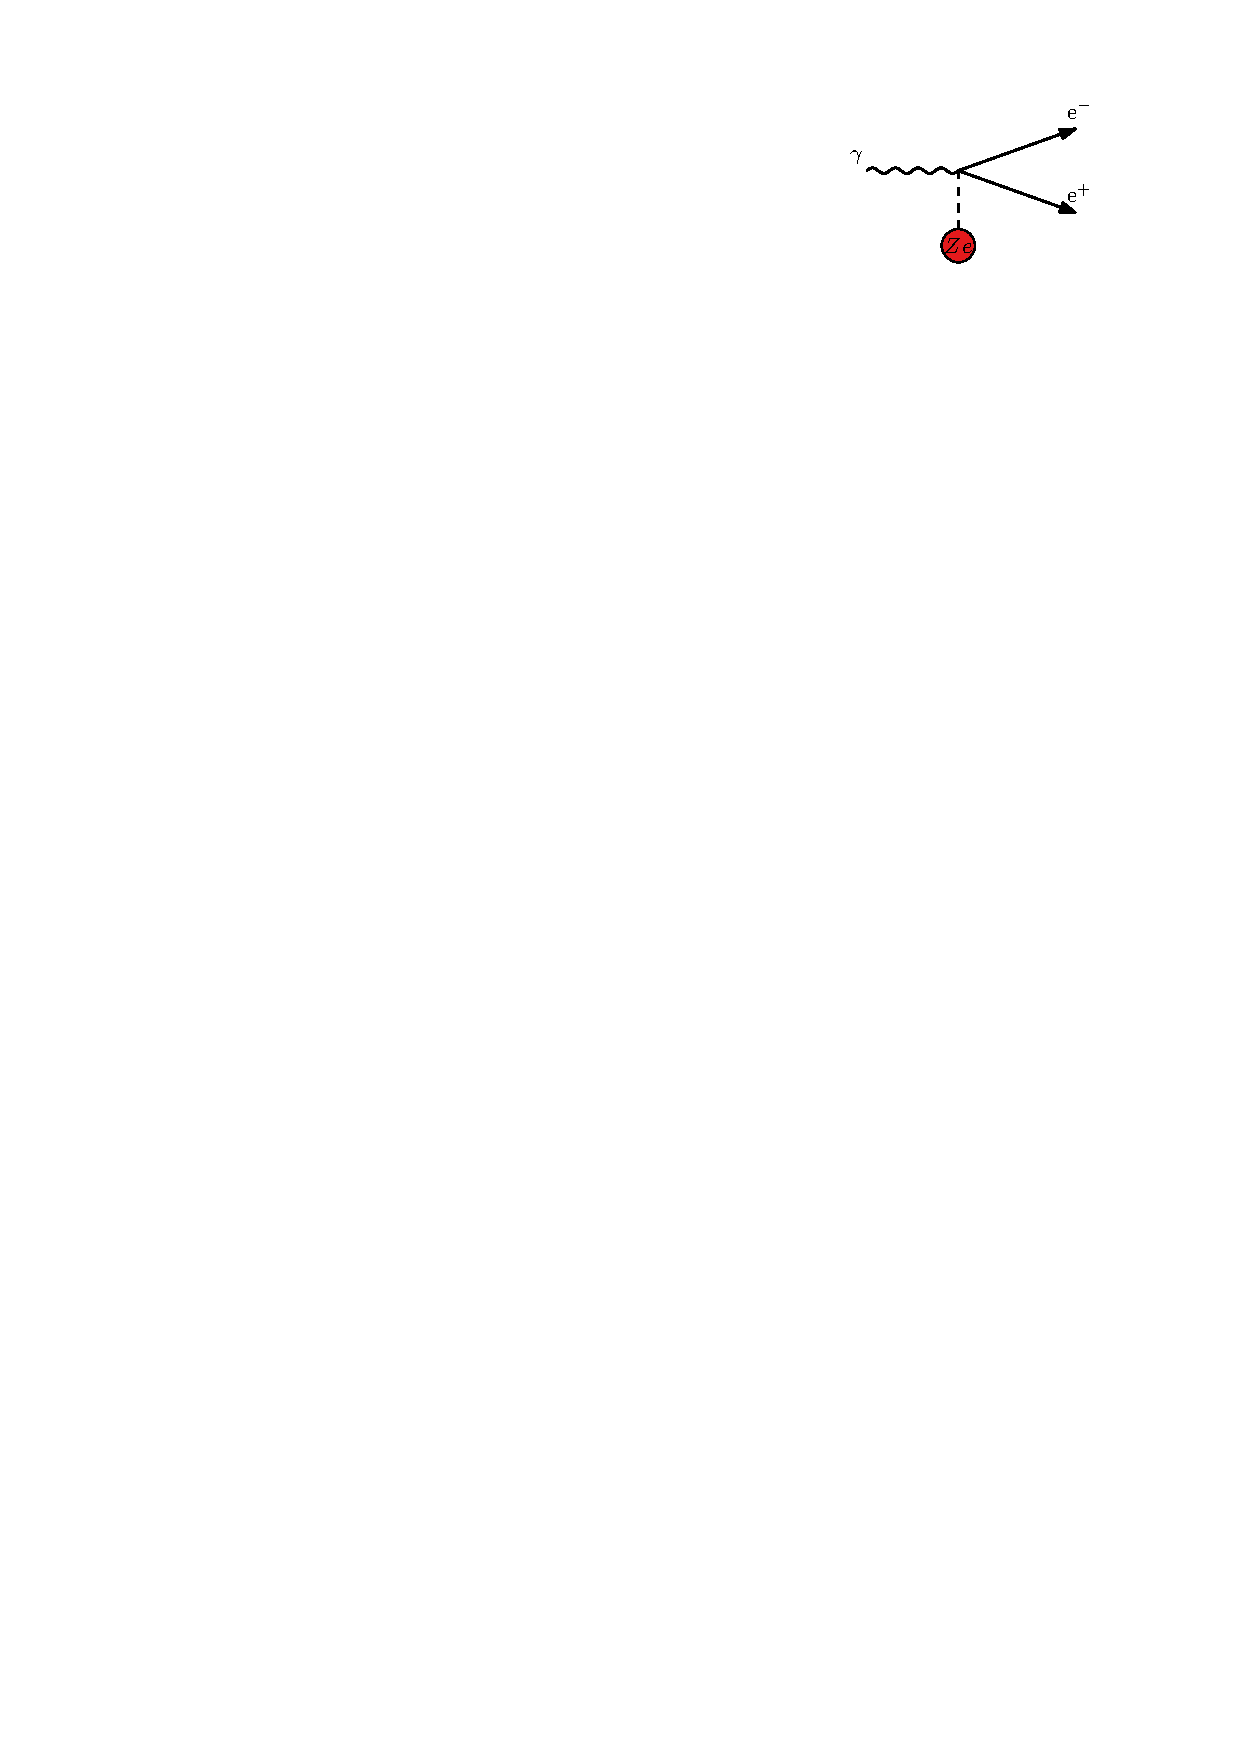
\includegraphics{./figures/pair_intro.pdf}
		\end{center}
		
		\column[c]{0.6\textwidth}
		Pair production
	\end{columns}
\end{frame}

\note[itemize]{
	\item (independent) proccesses relevant in energy range (\si{keV} -- \si{GeV}) for nuclear \& detector physics
	
	\item photoelectric effect:
	\begin{itemize}
		\item photon absorbed by atomic electron
		\item electron liberated
		\item dominant at low energies
	\end{itemize}
	
	\item compton scattering:
	\begin{itemize}
		\item scattering of photons at free / quasifree electrons
		\item dominant at intermediate energies
	\end{itemize}
	
	\item pair production:
	\begin{itemize}
		\item $\mathrm{e}^+ \mathrm{e}^-$ production in Coulomb field
		\item dominant at high energies
	\end{itemize}
	
	\item other processes:
	\begin{itemize}
		\item Thomson \& Rayleigh scattering (?)
	\end{itemize}
}

\begin{frame}{Introduction -- Lambert-Beer law}
	\begin{columns}
		\column[t]{0.6\textwidth}
		Photon beam passing through matter:
			\begin{itemize}
				\item interaction removes $\gamma$ from beam by absorption or scattering
				\begin{itemize}
					\item individual $\gamma$ do not lose energy
					\item beam intensity is attenuated
				\end{itemize}
				
				\item attenuation:
				\begin{align*}
					\mathrm{d} I = - \mu I \mathrm{d}x
				\end{align*}
				\begin{itemize}
					\item Lambert-Beer law:
					\begin{align*}
					I(x) = I_0 \, e^{-\mu x}
					\end{align*}
				\end{itemize}
				
				
				\item mean free path
				\begin{align*}
					\lambda = \frac{1}{\mu}
				\end{align*}
			\end{itemize}

		\column[t]{0.4\textwidth}		
			\begin{center}
				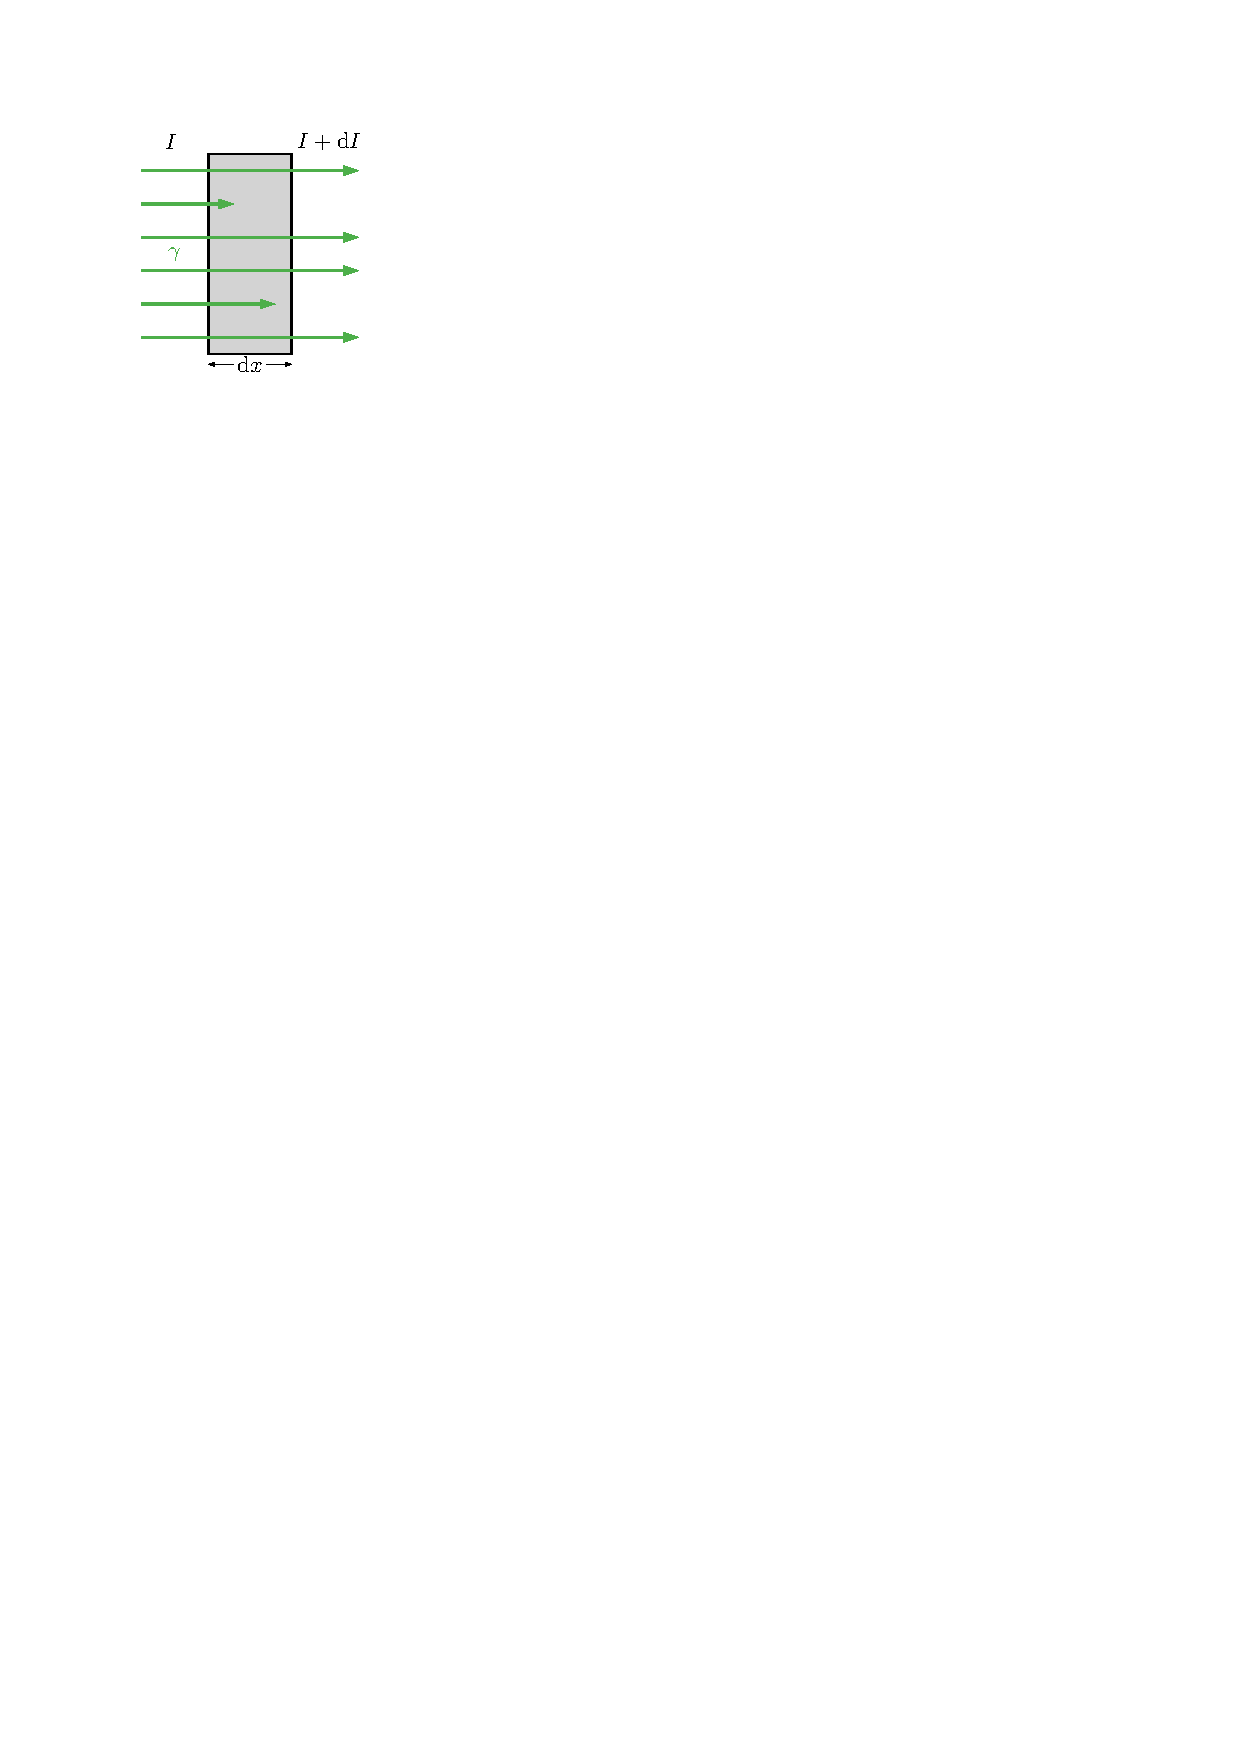
\includegraphics{./figures/lambert_beer.pdf}
			\end{center}			
	\end{columns}
\end{frame}

\note[itemize]{
	\item absorption coefficient material and energy dependent
}

\begin{frame}{Introduction -- range comparison}
	
	\begin{columns}
		\column[t]{0.5\textwidth}
		\centering
		\hspace{1cm}\textbf{charged particles:}
		
		\vspace{0.5cm}
		
		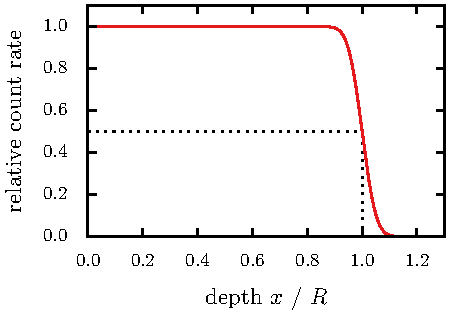
\includegraphics[width=1.0\textwidth]{./figures/range.pdf}
		
		\column[t]{0.5\textwidth}
		\centering
		\hspace{1cm}\textbf{photons:}
		
		\vspace{0.5cm}
		
		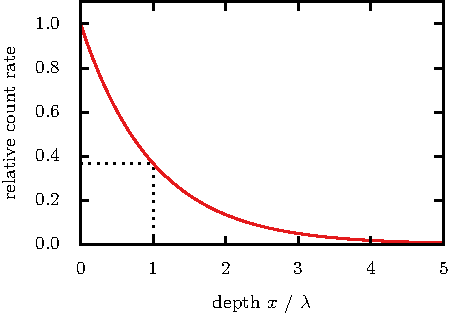
\includegraphics[width=1.0\textwidth]{./figures/lambert_beer_exp.pdf}
		
	\end{columns}
\end{frame}

\note[itemize]{
	\item charged particles gradually lose energy until stop at a fixed range
	\item photons don't lose energy but are absorbed or scattered from the beam	
}


\begin{frame}{Introduction - absorption coefficient}
	\begin{itemize}
		\setlength\itemsep{2.em}
		\item absorption coefficient
		\begin{align*}
			\mu = n \sigma
		\end{align*}
		$n$: density of atoms \\
		$\sigma$: total absorption/scattering cross section per atom
		
		\item cross section per atom
		\begin{align*}
			\sigma = \sigma_\mathrm{photo} + \sigma_\mathrm{Compton} + \sigma_\mathrm{pair}
		\end{align*}
		\begin{itemize}
			\item depends on material \& photon energy
		\end{itemize}		
	\end{itemize}	
\end{frame}

\note[itemize]{
	\item neglect other processes (processes independent)
	
	\item higher penetration power
	\begin{itemize}
		\item smaller cross section cmp.\ inelastic $\mathrm{e}^-$ collision
	\end{itemize} 
}

\begin{frame}{Introduction - absorption length}
	\begin{center}
		\begin{overpic}[width=1.0\textwidth]{./figures/absorption_length.pdf}
			\put(80, -4){\footnotesize \cite{pdg}}
		\end{overpic}
	\end{center}
\end{frame}

\note[itemize]{
	\item $n \propto \rho, \lambda \propto \frac{1}{n} \rightarrow \lambda \rho \propto \mathrm{const}$
	\item TODO: Why the deviation of hydrogen at $1 \mathrm{MeV}$?
	\item TODO: Why are the absorption lengths the same at $1 \mathrm{MeV}$? Where is the factor $Z$ from Compton scattering?
}

\section{Interaction processes}

\begin{frame}{Interaction processes -- overview}
	\centering
	\begin{overpic}[scale=0.9]{./figures/carbon.pdf}
		\put(80, -4){\footnotesize \cite{pdg}, modified}
	\end{overpic}
\end{frame}

\note[itemize]{
	\item $\sigma_\mathrm{Compton}$ -- per atom (not electron)
	
	\begin{itemize}
		\item photoelectric effect: $E_\gamma < \SI{1}{MeV}$
		\item Compton scattering: $E_\gamma \approx \SI{1}{MeV}$
		\item pair production: $E_\gamma > \SI{1}{MeV}$
	\end{itemize}
}

\subsection{Photoelectric effect}

\begin{frame}{Photoelectric effect}
	\begin{columns}
		\column[t]{0.6\textwidth}
		\begin{itemize}
			\setlength\itemsep{1.5em}
			\item dominant for $E_\gamma \ll 1 \, \mathrm{MeV}$
			
			\item absorption of $\gamma$ by atomic $\mathrm{e}^-$
			\begin{itemize}
				\item nucleus absorbs recoil momentum
			\end{itemize}
			
			\item threshold energy
			\begin{align*}
				E_\gamma > E_\mathrm{b}
			\end{align*}

			\item kinetic energy of $\mathrm{e}^-$ (neglect recoil)
			\begin{align*}
				T_\mathrm{e} = E_\gamma - E_\mathrm{b}
			\end{align*}
		\end{itemize}
		
		\column[t]{0.4\textwidth}
		\begin{center}
			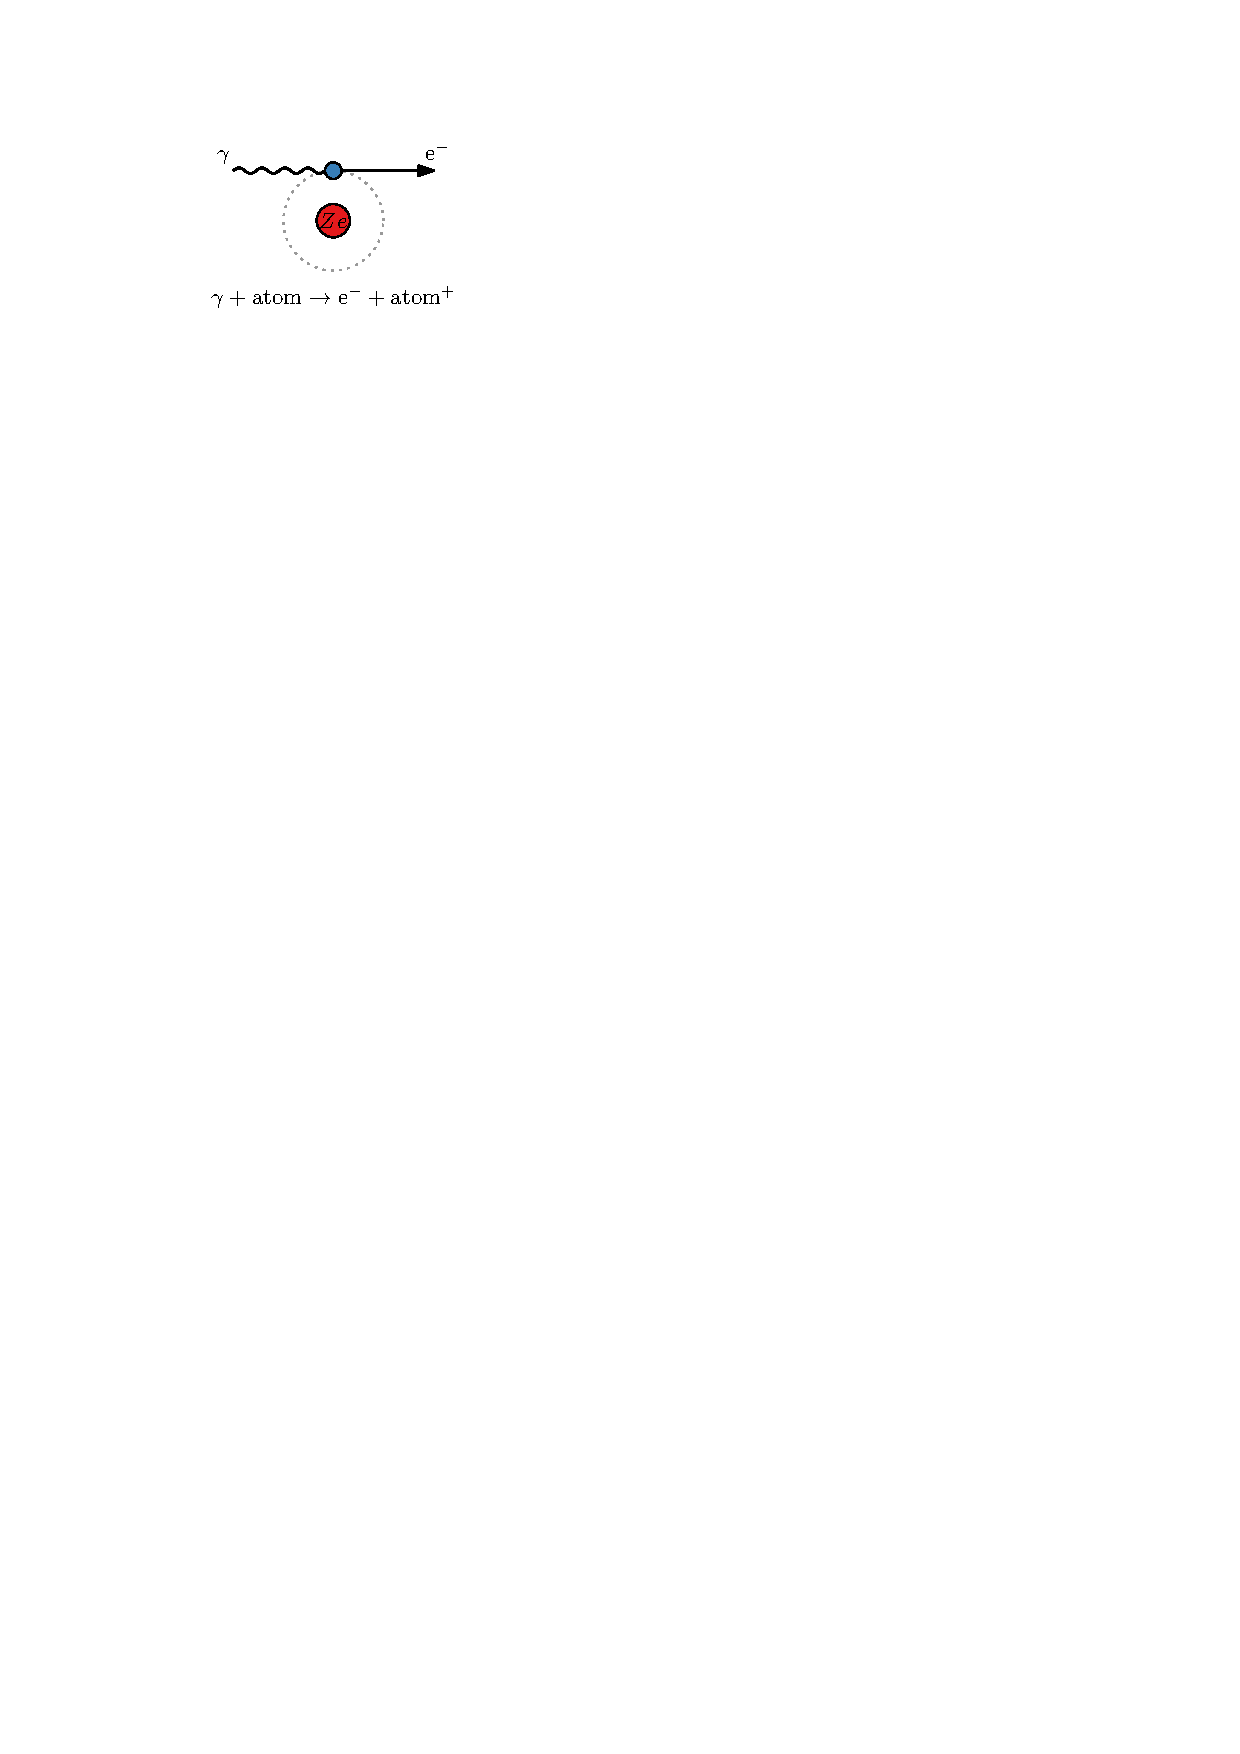
\includegraphics{./figures/photoeffect_detail.pdf}
		\end{center}
	\end{columns}
\end{frame}

\note[itemize]{
	\item complete transfer of energy
	\item nucleus required because of 4-momentum conservation
	\item binding energy depends on atomic shell
	\item recoil can be neglected since nucleus is heavy compared to electron
}

\begin{frame}{Photoelectric effect -- shell structure}
	\begin{columns}
		\column[c]{0.55\textwidth}
		\begin{itemize}
			\setlength\itemsep{1.5em}
			\item $\sigma_\mathrm{photo}$ increases with increasing binding energy $E_\mathrm{b}$ of the electron
			
			\item atomic shell structure visible
			\begin{itemize}
				\item absorption edges
			\end{itemize}
			
			\item K-shell dominant
			\begin{align*}
				\frac{\sigma_\mathrm{K}}{\sigma_\mathrm{L}} = 5 - 13
			\end{align*}
		\end{itemize}
		
		\column[c]{0.45\textwidth}
		\begin{overpic}[width=1.0\textwidth]{./figures/lead_edges.png}
			\put(20,20){\footnotesize \rmfamily Lead ($Z=82$)}
			\put(39, -1){\footnotesize $E_\gamma \, / \, \mathrm{MeV}$}
			\put(-2, 40){\rotatebox{90}{\footnotesize $\sigma_\mathrm{photo} \, / \, \mathrm{barn}$}}
			\put(32, 80){\footnotesize \rmfamily K-Edge ($E_\gamma \approx 88 \, \mathrm{keV}$)}
			\put(18, 94){\footnotesize \rmfamily L-Edges}
			\put(60, -10){\footnotesize \cite{leo}, modified}
		\end{overpic}
	\end{columns}
\end{frame}

\note[itemize]{
	\item
}

\begin{frame}{Photoelectric effect -- cross section}
	\begin{itemize}
		\setlength\itemsep{1.5em}
		\item exact solution difficult
		\begin{itemize}
			\item infinite number of partial waves
		\end{itemize}
		\item approximate solution
		\begin{itemize}
			\item only K-shell electrons
			\item non-relativistic final state electron			
			\begin{align*}
				&\sigma_\mathrm{photo} = \underbrace{4\sqrt{2} \alpha^4 \sigma_\mathrm{Th} \alert{Z^5}  \left( \frac{m_\mathrm{e}c^2}{\alert{E_\gamma}} \right)^{\alert{\frac{7}{2}}}}_{\text{Born approximation}} \cdot \, \overbrace{f(Z, E_\gamma)}^{\mathclap{\substack{\text{correction}\\\text{near K-edge}}}} \\[1em]
				&\sigma_\mathrm{Th}\text{: Thomson cross section}
			\end{align*}
		\end{itemize}
	\end{itemize}
\end{frame}

\note[itemize]{
	\item $E_\mathrm{b}^\mathrm{K} < E_\gamma \ll m_\mathrm{e}c^2$
	\item only K-shell justified -- other shells negligible
	\item photon energies less than electron rest mass
	\item Born approximation: final state electron -- plane wave (neglects influence of nucleus)
	\item near K-edge nucleus important: correction factor depending on $Z$ and $E_\gamma$
	
	\item TODO: whats near the K-edge? how big is the correction?
}

\begin{frame}{Photoelectric effect -- dependencies}
	\begin{itemize}
		\setlength\itemsep{1.5em}
		\item non-relativistic case (incl.\ correction)
		\begin{align*}
		\sigma_\mathrm{photo} \propto  \frac{Z^{4 \, \dots \, 5}}{E_\gamma^{n}} \qquad n \leq \frac{7}{2}
		\end{align*}
		
		\item relativistic case
		\begin{align*}
			\sigma_\mathrm{photo} \propto \frac{Z^5}{E_\gamma}
		\end{align*}
		\begin{itemize}
			\item non-rel.\ approximation generally sufficient -- Compton scattering
		\end{itemize} 
	\end{itemize}
\end{frame}

\note[itemize]{
	\item non-rel.\ case: correction important for low photon energies
	
	\item relativistic case: consider Dirac final state wavefunctions
	
	\item generally at energies \SI{250}{keV}, where relativistic effects become important -- Compton scattering is becoming the  dominant interaction
	
	\item Photoeffect important for low $E$ high $Z$ -- Detectors build from high $Z$ material / Lead-shielding
	
	\item Angular distribution: low E -- \SI{90}{\degree} (dipole radiation), high E -- forward direction (?)
}


\subsection{Compton scattering}

\begin{frame}{Interaction processes -- overview}
	\centering
	\begin{overpic}[scale=0.9]{./figures/carbon.pdf}
		\put(80, -4){\footnotesize \cite{pdg}, modified}
	\end{overpic}
\end{frame}

\begin{frame}{Compton scattering}
\begin{columns}
	\column[t]{0.6\textwidth}
	\begin{itemize}
		\setlength\itemsep{1.5em}
		\item dominant for $E_\gamma \approx 1 \, \mathrm{MeV}$
		
		\item scattering of photon at free electron
		\begin{itemize}
			\item quasi-free for $E_\gamma \gg E_\mathrm{b}$
		\end{itemize}
		
		\item energy transfer from 4-momentum conservation
		\begin{align*}
			T_\mathrm{e} = E_\gamma \frac{\epsilon (1 - \cos\theta)}{1 + \epsilon (1 - \cos\theta)} \qquad \epsilon := \frac{E_\gamma}{m_\mathrm{e}c^2}
		\end{align*}
		\begin{itemize}
			\item maximum for backscattering (Compton edge)
			\begin{align*}
				T_\mathrm{e, max} = E_\gamma \frac{2\epsilon}{1+ 2\epsilon}
			\end{align*}
		\end{itemize}
		
	\end{itemize}
	
	\column[t]{0.4\textwidth}
	\begin{center}
		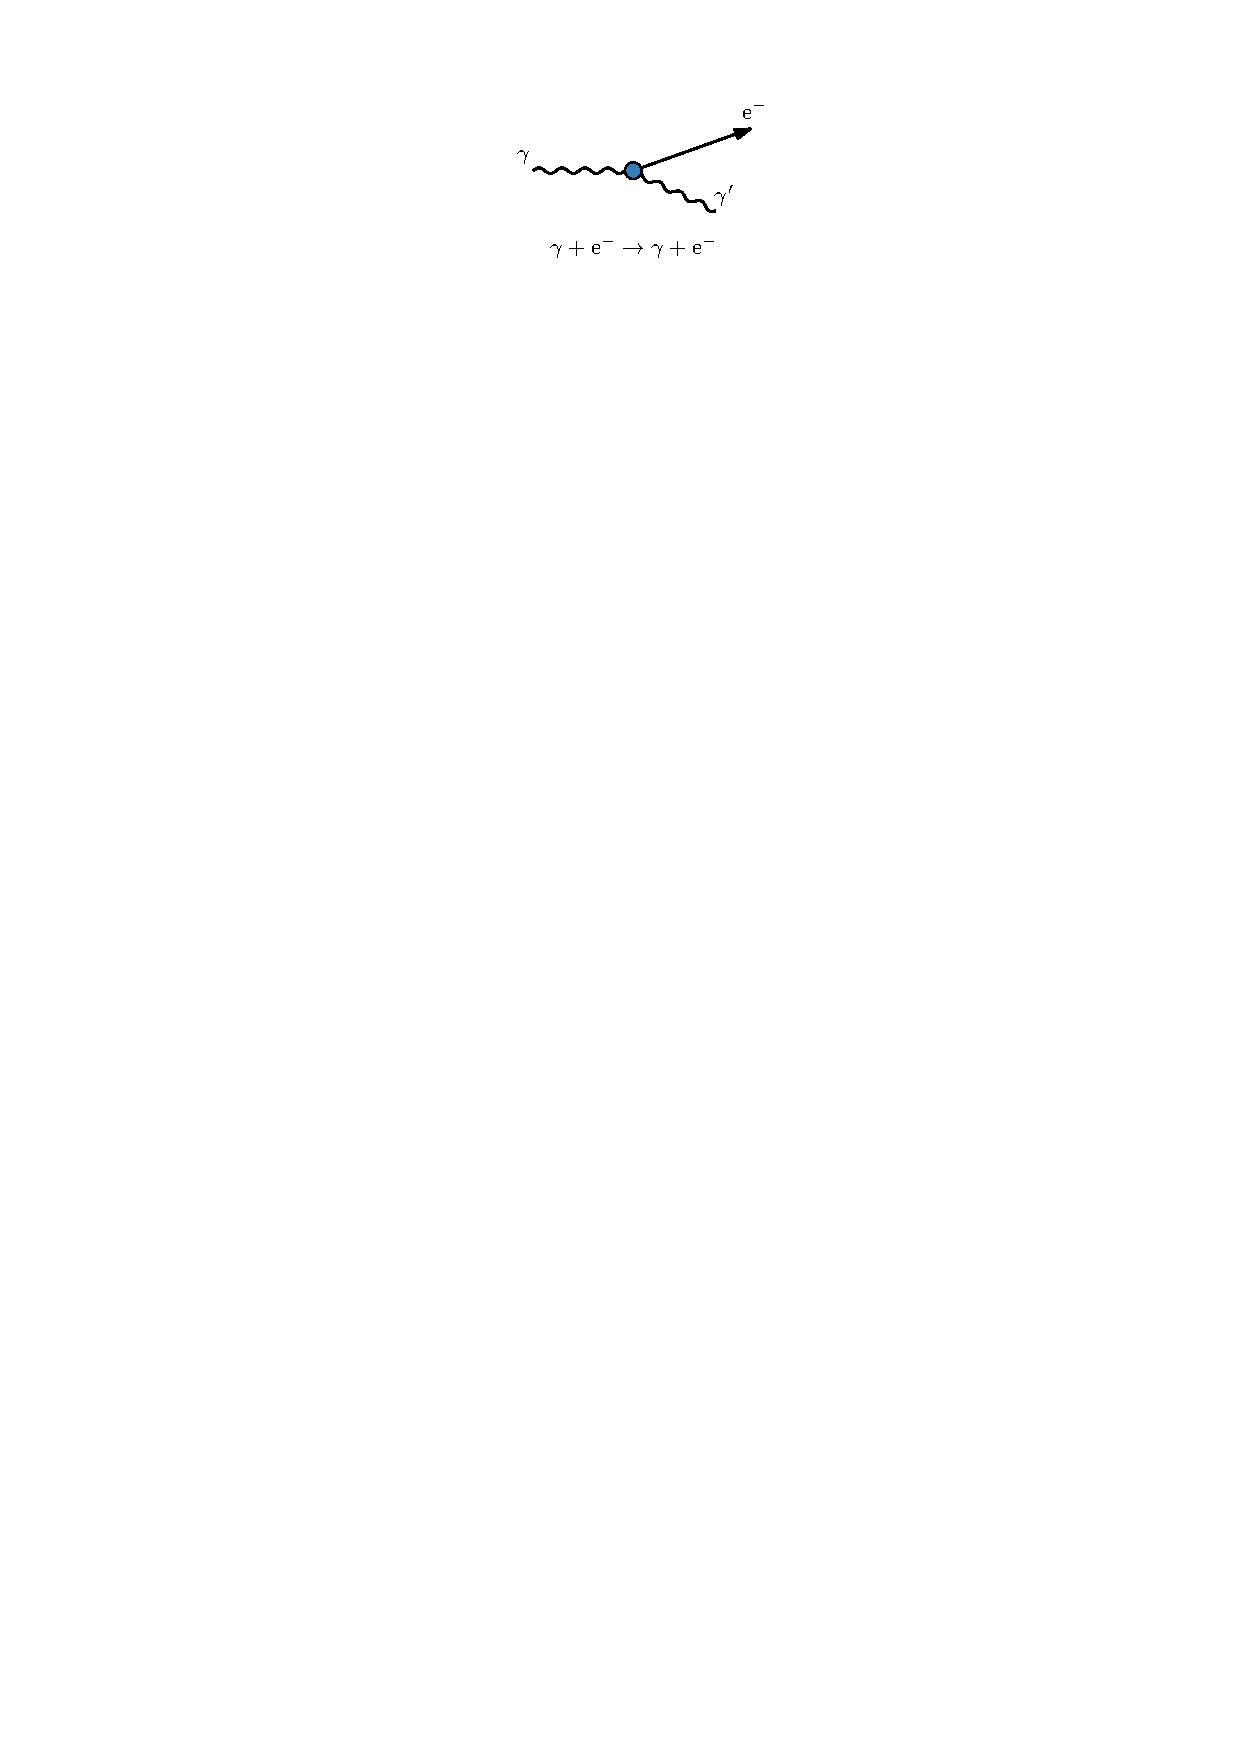
\includegraphics{./figures/compton_detail.pdf}
	\end{center}
\end{columns}
\end{frame}

\note[itemize]{
	\item results for single electrons
	\item larger dominant range for small $Z$
	\item Energy of scattered photon
	\begin{align*}
	E_\gamma^\prime = \frac{E_\gamma}{1 + \epsilon (1 - \cos\theta)} \\
	\end{align*}
	
}

\begin{frame}{Compton scattering -- diff.\ cross section}
	\begin{columns}
		\column[t]{0.55\textwidth}
		\begin{itemize}
			\setlength\itemsep{1.5em}
			\item Thomson cross section
				\begin{align*}
				\sigma_\mathrm{Th} = \frac{8 \pi}{3} r_\mathrm{e}^2
				\end{align*}
				
			\item advent of QED -- Klein-Nishina (1928)
			\begin{align*}
				P(E_\gamma, \theta) := \frac{E_\gamma^\prime(E_\gamma, \theta)}{E_\gamma}
			\end{align*}
		\end{itemize}
		
		\column[t]{0.45\textwidth}
		\begin{center}
			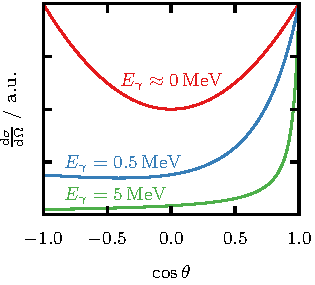
\includegraphics{./figures/compton_angular.pdf}
		\end{center}		
	\end{columns}
						
	\begin{align*}
	\frac{\mathrm{d}\sigma}{\mathrm{d}\Omega} = \frac{r_\mathrm{e}^2}{2} \cdot P(E_\gamma, \theta)^2 \bigg[ P(E_\gamma, \theta) + \frac{1}{P(E_\gamma, \theta)} + \cos^2\theta - 1 \bigg]
	\end{align*}
\end{frame}

\note[itemize]{
	\item Thomson -- $\sigma_\mathrm{Th} = \frac{8 \pi}{3} r^2$ -- strong deviation
	\item classical electron radius: $r_\mathrm{e} = \SI{2.8}{fm}$
	\item J.J.\ Thomson -- discovery of electron using cathode rays
	\item one of the first results of QED: Klein-Nishina
	\item Thomson reproduced in low energy limit
	\begin{itemize}
		\item low energy limit for photons propagating through matter - Rayleigh scattering (coherent scattering at bound electrons)
	\end{itemize}
	\item unpolarized photons
}


\begin{frame}{Compton scattering -- diff.\ cross section}
	\begin{columns}
		\column[c]{0.55\textwidth}
		\begin{itemize}
			\setlength\itemsep{1.5em}
			\item generally interested in energy transfer
			\begin{align*}
				\frac{\mathrm{d} \sigma}{\mathrm{d} T_\mathrm{e}} = \left(\frac{\mathrm{d}T_\mathrm{e}}{\mathrm{d}\cos\theta}\right)^{-1} \cdot 2 \pi \frac{\mathrm{d}\sigma}{\mathrm{d}\Omega}
			\end{align*}
		\end{itemize}
		
		\column[c]{0.45\textwidth}
		\begin{center}
			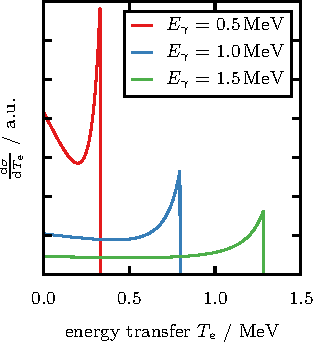
\includegraphics{./figures/compton_energytrans.pdf}
		\end{center}		
	\end{columns}
\end{frame}

\note[itemize]{
	\item in detector physics: measure deposited energy
	\item differential cross section w.r.t.\ $T$ using substitution
	\item increased probability of high energy transfer
	\item compton-edge clearly visible
	\item shifted to higher energies for higher $E_\gamma$
}

\begin{frame}{Compton scattering -- cross section}
	\begin{itemize}
		\setlength\itemsep{1.5em}
		\item classical limit -- $(\epsilon \ll 1)$
		\begin{align*}
			\sigma = \sigma_\mathrm{Th} \cdot (1 - 2 \epsilon)
		\end{align*}
		\item ultrarelativistic limit -- $(\epsilon \gg 1)$
		\begin{align*}
			\sigma = \frac{3}{8} \sigma_\mathrm{Th} \cdot \frac{1}{\alert{\epsilon}} \left( \frac{1}{2} + \alert{\ln(2\epsilon)} \right)
		\end{align*}
		\begin{itemize}
			\item decreases as
			\begin{align*}
				\sigma \sim \frac{1}{E_\gamma}
			\end{align*}
		\end{itemize}
		
		\item $Z$ electrons per atom
		\begin{align*}
			\sigma_\mathrm{Compton} = \alert{Z} \cdot \sigma
		\end{align*}
	\end{itemize}
\end{frame}


\subsection{Pair production}

\begin{frame}{Interaction processes -- overview}
	\centering
	\begin{overpic}[scale=0.9]{./figures/carbon.pdf}
		\put(80, -4){\footnotesize \cite{pdg}, modified}
	\end{overpic}
\end{frame}

\note[itemize]{
	\item $\sigma_\mathrm{Th} = \SI{0.66}{b}$
	\item $Z \cdot \sigma_\mathrm{Th}$ approx.\ maximum of $\sigma_\mathrm{Compton}$ in PDG-Plot
	\item only Compton effect -- expect constant cross section at low energies (Thomson)
	\begin{itemize}
		\item Rayleigh scattering replaces Compton
		\item Rayleigh coherent scattering at all electrons of the atom
		\item wavelength large -- can't resolve single electrons
		\item negligible energy transfer -- not relevant for detector physics
	\end{itemize}
}

\begin{frame}{Pair production}
\begin{columns}
	\column[t]{0.6\textwidth}
	\begin{itemize}
		\setlength\itemsep{1.5em}
		\item dominant for $E_\gamma \gg 1 \, \mathrm{MeV}$
		
		\item creation of $\mathrm{e}^- \mathrm{e}^+$-pair in a Coulomb field
		\begin{itemize}
			\item 4-momentum conservation requires third body (nucleus or electron)
			\item generally negligible for electrons
			\begin{align*}
				\frac{\sigma_\mathrm{pair,\, nuc}}{\sigma_\mathrm{pair,\, e}} \approx Z
			\end{align*}
		\end{itemize}
		
		\item threshold energy (neglecting recoil)
		\begin{align*}
			E_\gamma > 2 m_\mathrm{e}c^2
		\end{align*}
		
		
	\end{itemize}
	
	\column[t]{0.4\textwidth}
	\begin{center}
		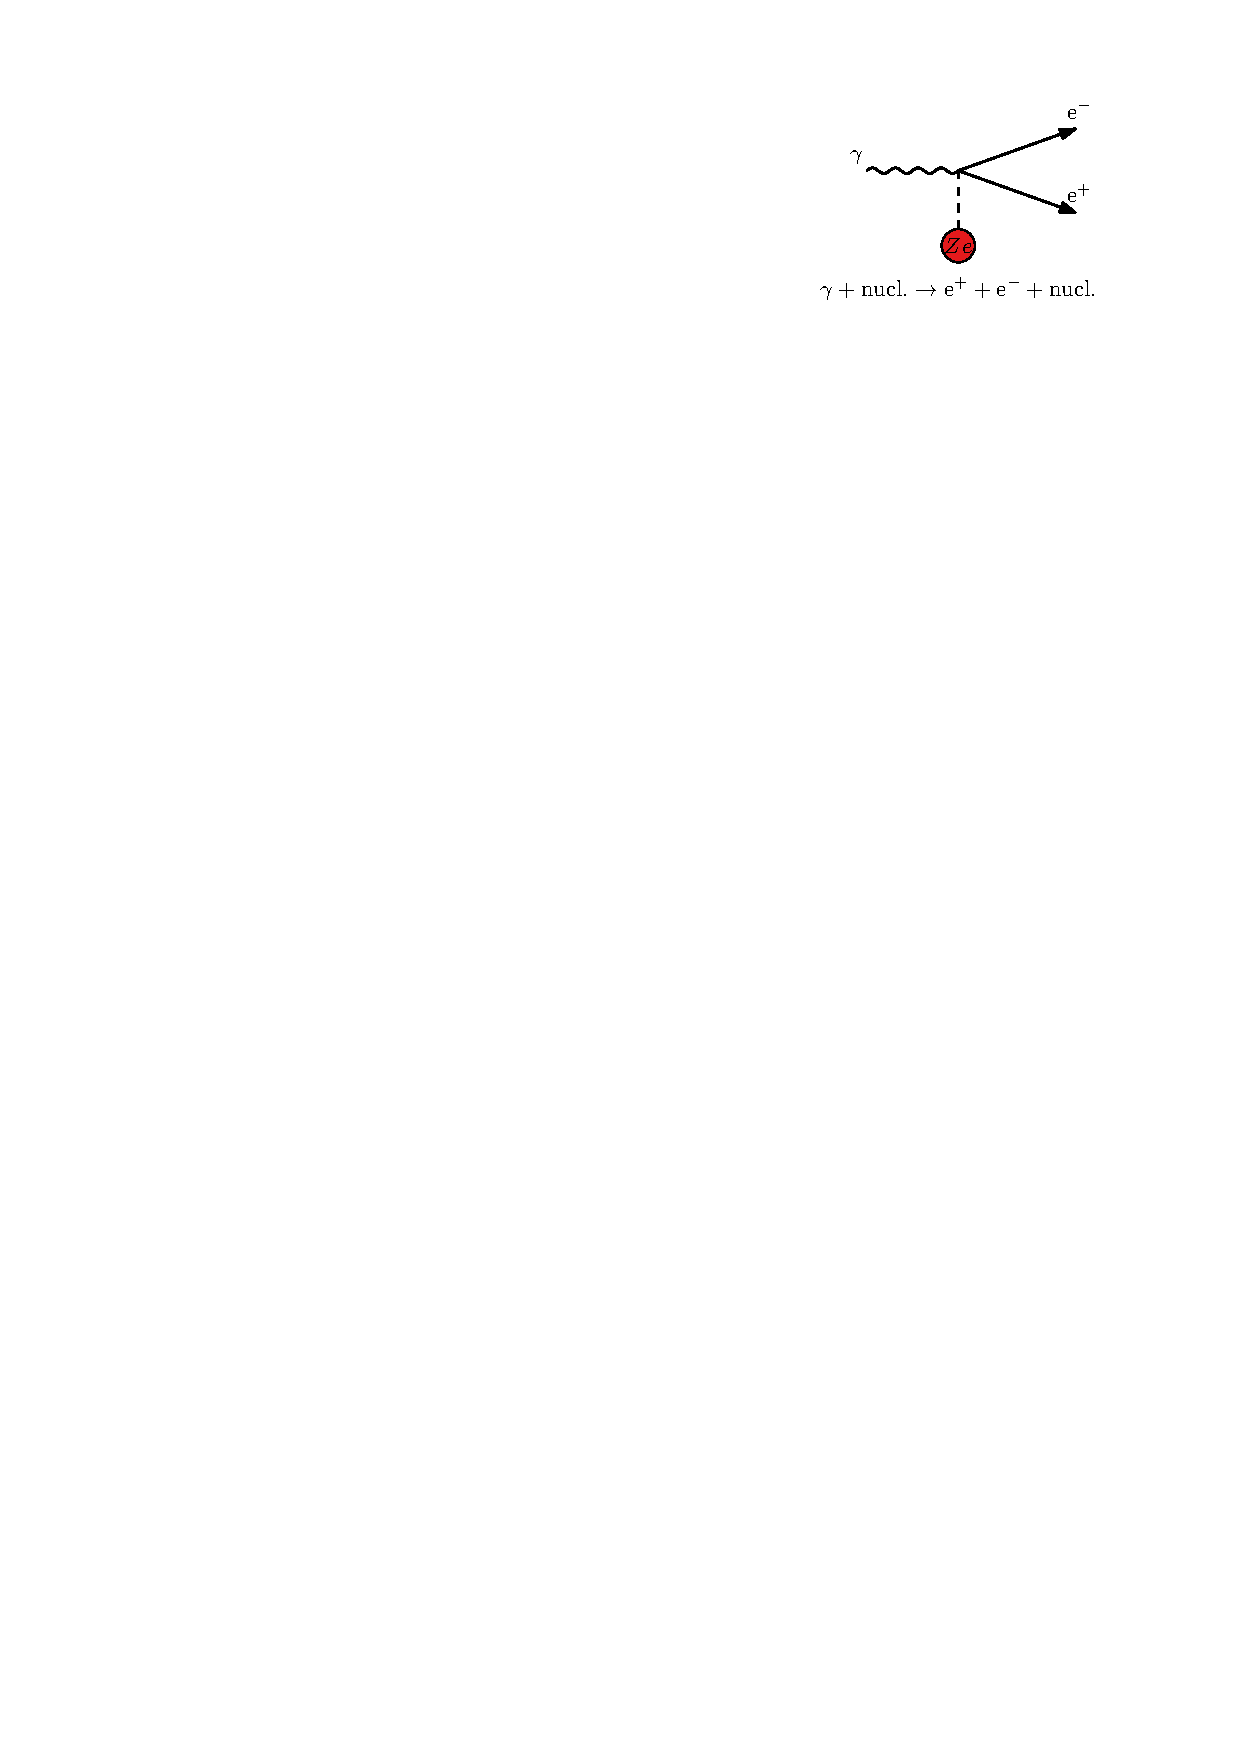
\includegraphics{./figures/pair_detail.pdf}
	\end{center}
\end{columns}
\end{frame}

\note[itemize]{
	\item Proof (momentum conservation):
	\begin{align*}
		&k = p_1 + p_2 \rightarrow k^2 = (p_1 + p_2)^2 = 0 \\
		&0 = 2 m_\mathrm{e}^2 + 2 (E_1 E_2 - \vec{p}_1 \cdot \vec{p}_2) \geq 2 m_\mathrm{e}^2
	\end{align*}
	
	\item pair production in field of electron only significant for light particles -- detectors generally large $Z$
	
	\item threshold energy larger for electrons -- larger recoil energy due to smaller mass
	\begin{itemize}
		\item has to be considered for low $Z$
	\end{itemize}
}

\begin{frame}{Pair production -- relation to bremsstrahlung}
	\begin{itemize}
		\setlength\itemsep{1.5em}
		\item related to bremsstrahlung by crossing symmetry
		
		\begin{center}
			\vspace{0.3cm}
			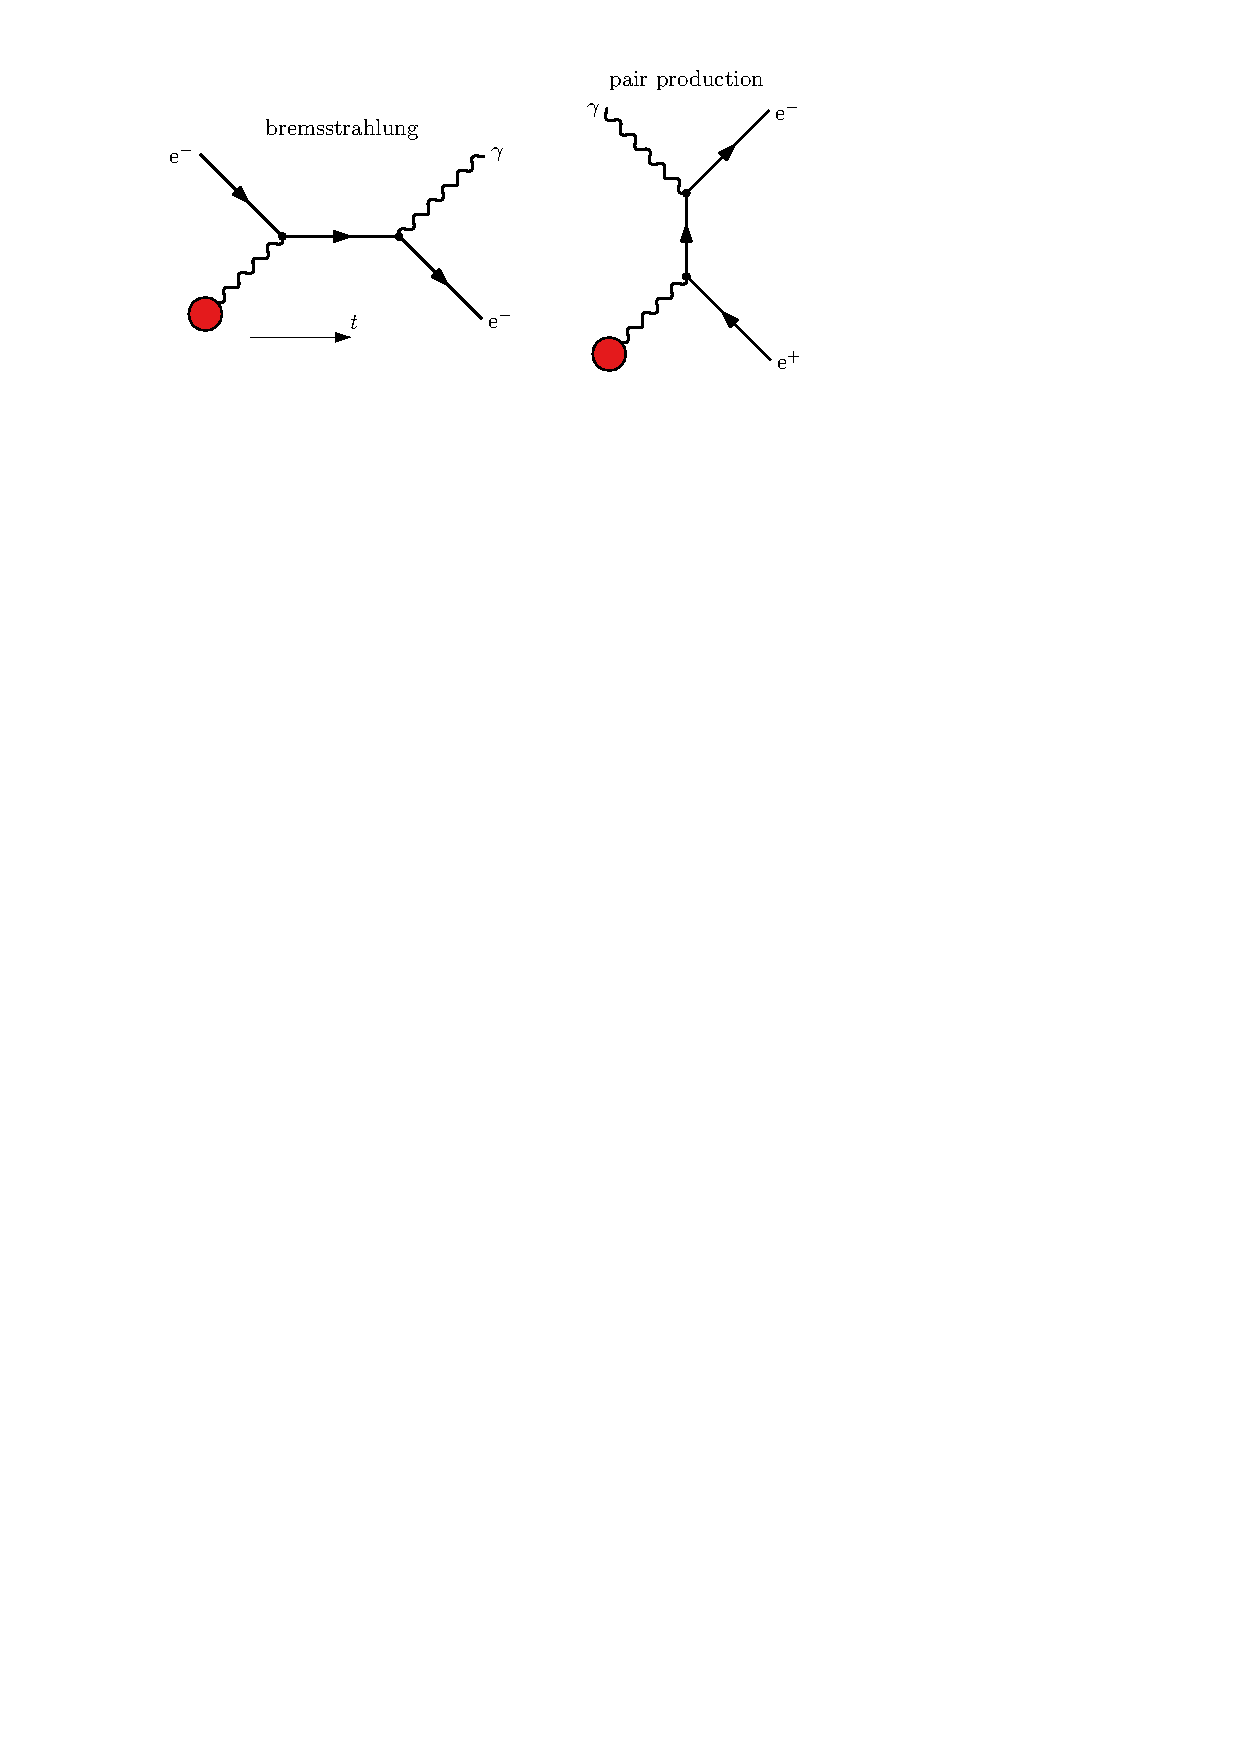
\includegraphics[width=0.9\textwidth]{./figures/crossing_symmetry.pdf}
		\end{center}
		
		\item radiation length~$X_0$ will be characteristic of the mean free path of pair production
		\begin{align*}
			\lambda_\mathrm{pair} \propto X_0
		\end{align*}
	\end{itemize}
\end{frame}

\begin{frame}{Pair production -- cross section}
	\begin{itemize}
		\setlength\itemsep{1.5em}
		\item charge of nucleus is screened by atomic electrons
		\begin{itemize}
			\item screening decreases with increasing momentum transfer $q^2$
		\end{itemize}
		
		\item for $E_\gamma \gg m_\mathrm{e} c^2$ (complete screening)
		\begin{align*}
			\sigma_\mathrm{pair} &= \frac{7}{9} \frac{1}{X_0} \frac{A}{N_\mathrm{A} \rho}
		\end{align*}
		
		\item approximate proportionality $\sigma_\mathrm{pair} \propto Z^2$
		\begin{itemize}
			\item independent of $E_\gamma$
		\end{itemize}
		
		\item characteristic length of pair production
			\begin{align*}
				\lambda_\mathrm{pair} = \frac{1}{n \, \sigma_\mathrm{pair}} = \frac{9}{7} X_0
			\end{align*}
	\end{itemize}
\end{frame}

\note[itemize]{
	\item probability distribution for $q^2$ shows that for high $E_\gamma$ smaller $q^2$ are more probable (and vice versa)
	\begin{itemize}
		\item less screening at low energies (high $q^2$)
		\item complete screening at high energies (small $q^2$)
	\end{itemize}
	
	\item complete screening good for $E_\gamma = \mathcal{O}(100 \, \mathrm{MeV} - 1 \, \mathrm{GeV})$
	\begin{itemize}
		\item atomic mass $A$ in \si{g\per\mole}
		\item mass density $\rho$
		\item avogadros number $N_\mathrm{A}$
		\item radiation length $X_0$ in $\mathrm{cm}$
	\end{itemize}
	
	\item over a distance of $X_0$
	\begin{itemize}
		\item an electron loses $63\, \si{\percent}$ of its energy due to bremsstrahlung
		\item a photon has a probability of $54 \si{\percent}$ to perform pair production
	\end{itemize}
	
	\item LPM effect (?)
}

\begin{frame}{Interaction processes -- dependencies of the cross section}
	\begin{center}
		\begin{tabular}{ccc}
			\toprule
			& atomic number $Z$ & photon energy $E_\gamma$\\
			\midrule
			\begin{minipage}{0.3\textwidth}
				\centering
				\textbf{photoelectric effect}
				
				\vspace{0.1cm}
				
				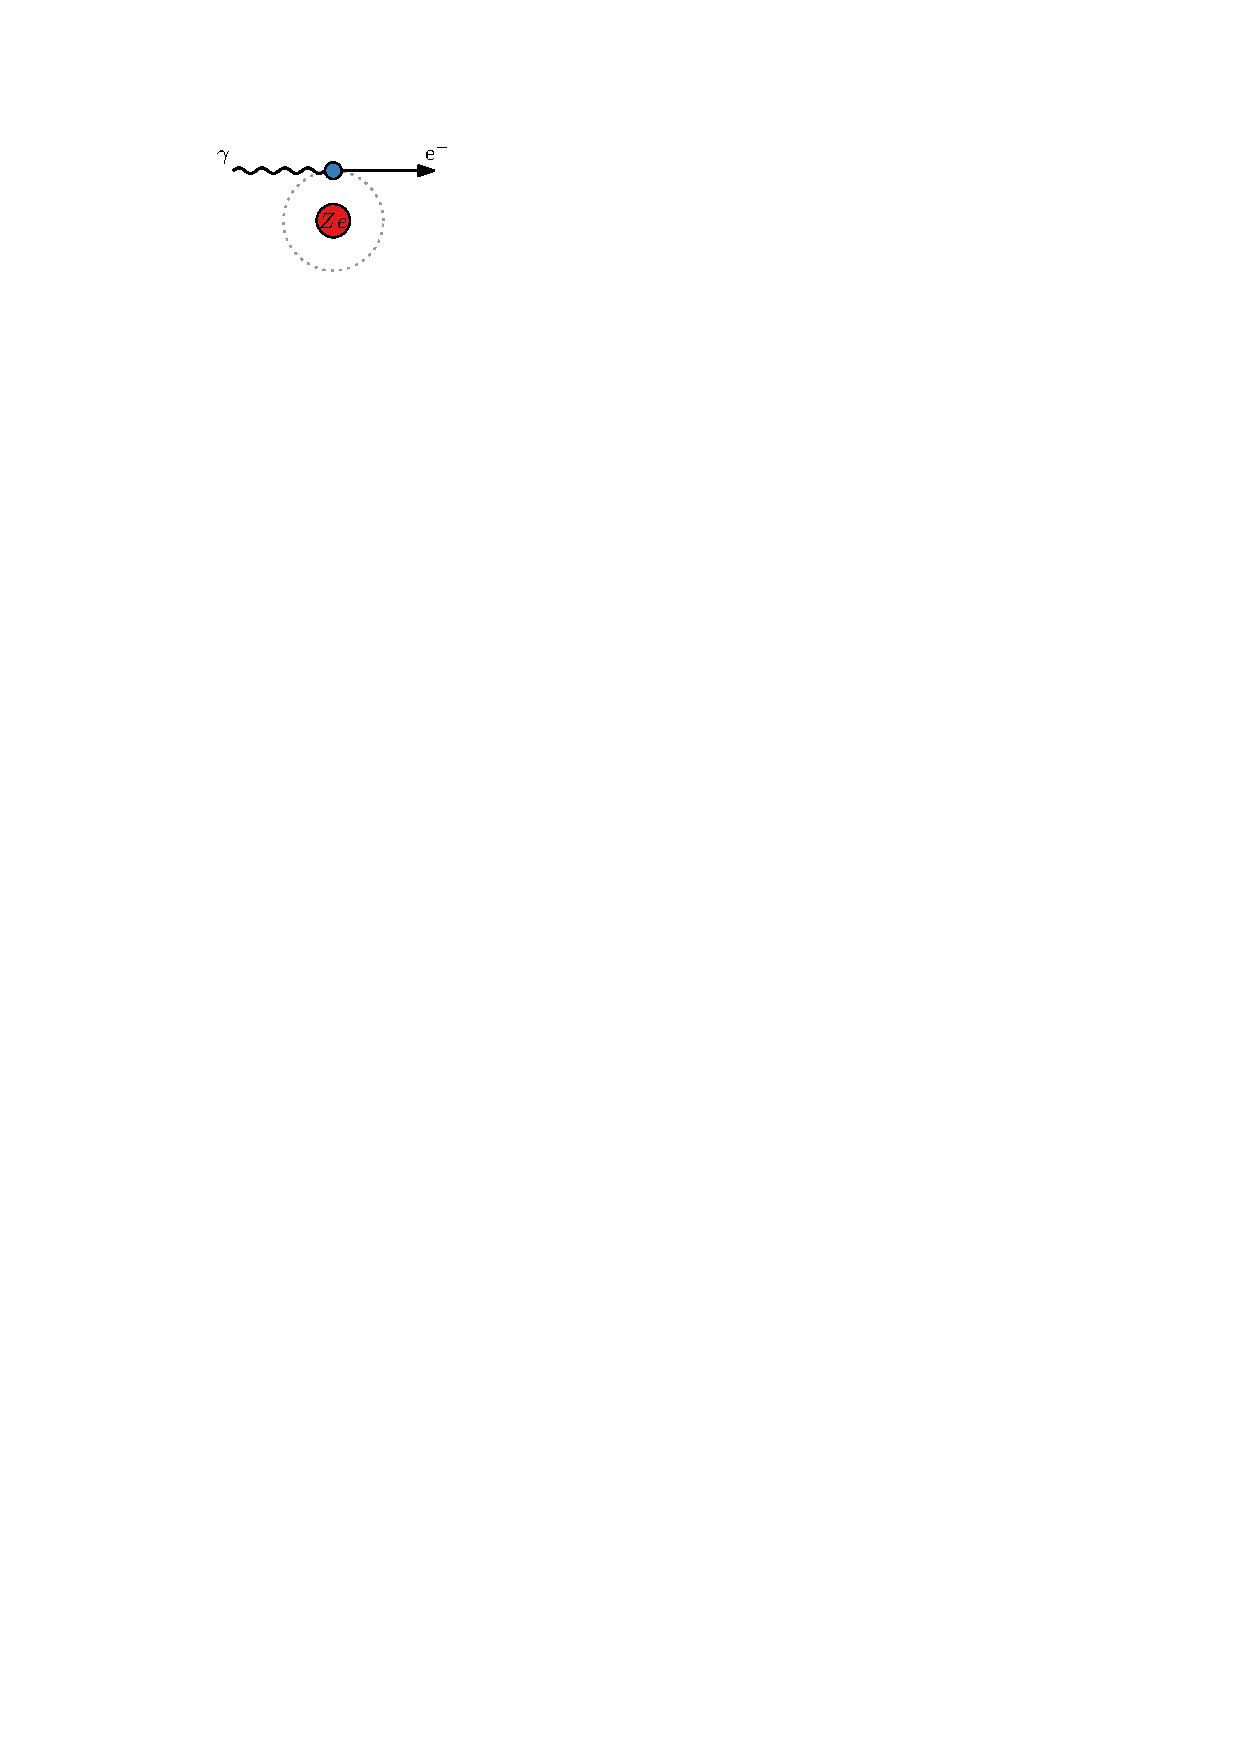
\includegraphics[width=0.8\textwidth]{./figures/photoeffect_intro.pdf} 
				
				\vspace{0.4cm}
			\end{minipage} & $Z^5$ & $E_\gamma^{-\frac{7}{2}}$ \\
			
			\begin{minipage}{0.3\textwidth}
				\centering
				\textbf{Compton scattering}
				
				\vspace{0.1cm}
				
				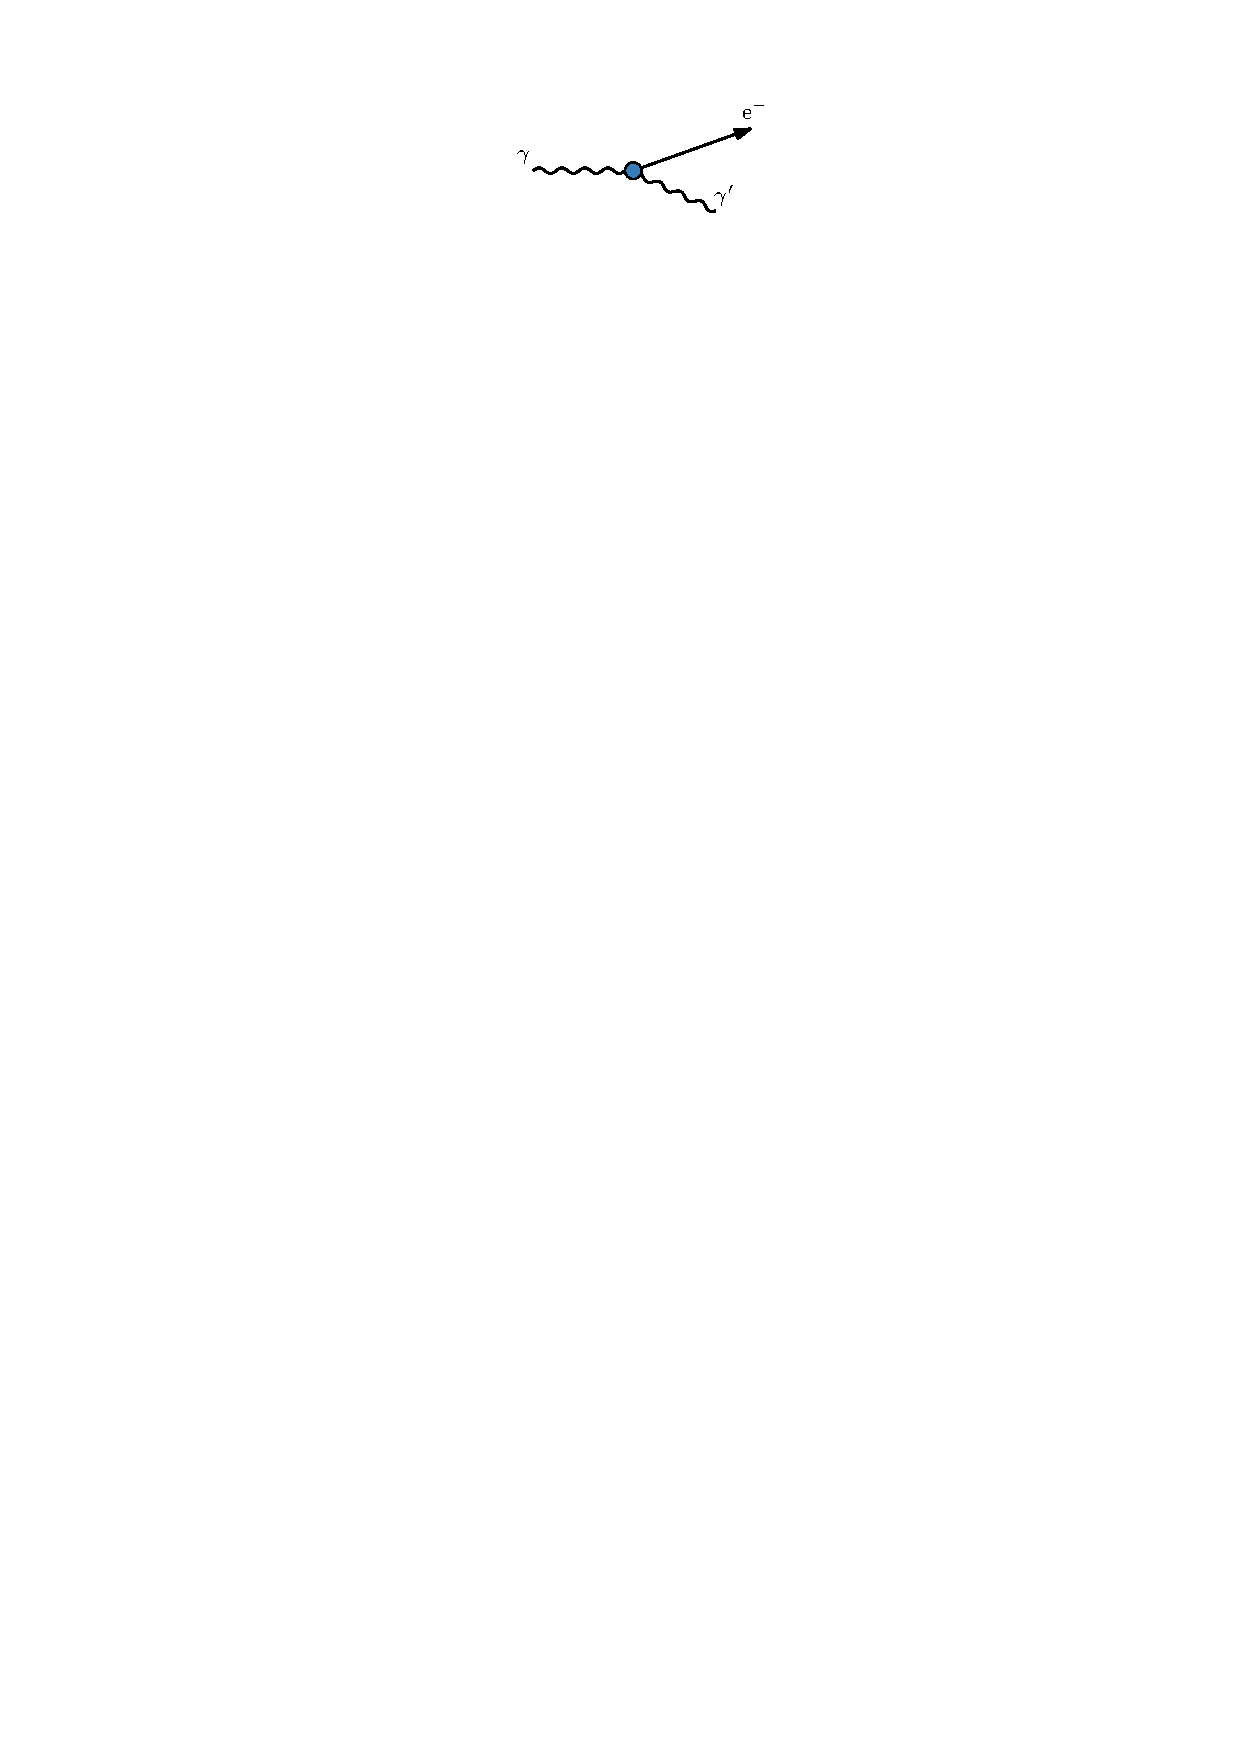
\includegraphics[width=0.8\textwidth]{./figures/compton_intro.pdf} 
				
				\vspace{0.4cm}
			\end{minipage} & $Z$ & $\frac{1}{E_\gamma}$\\
			
			\begin{minipage}{0.3\textwidth}
				\centering
				\textbf{pair production}
				
				\vspace{0.1cm}
				
				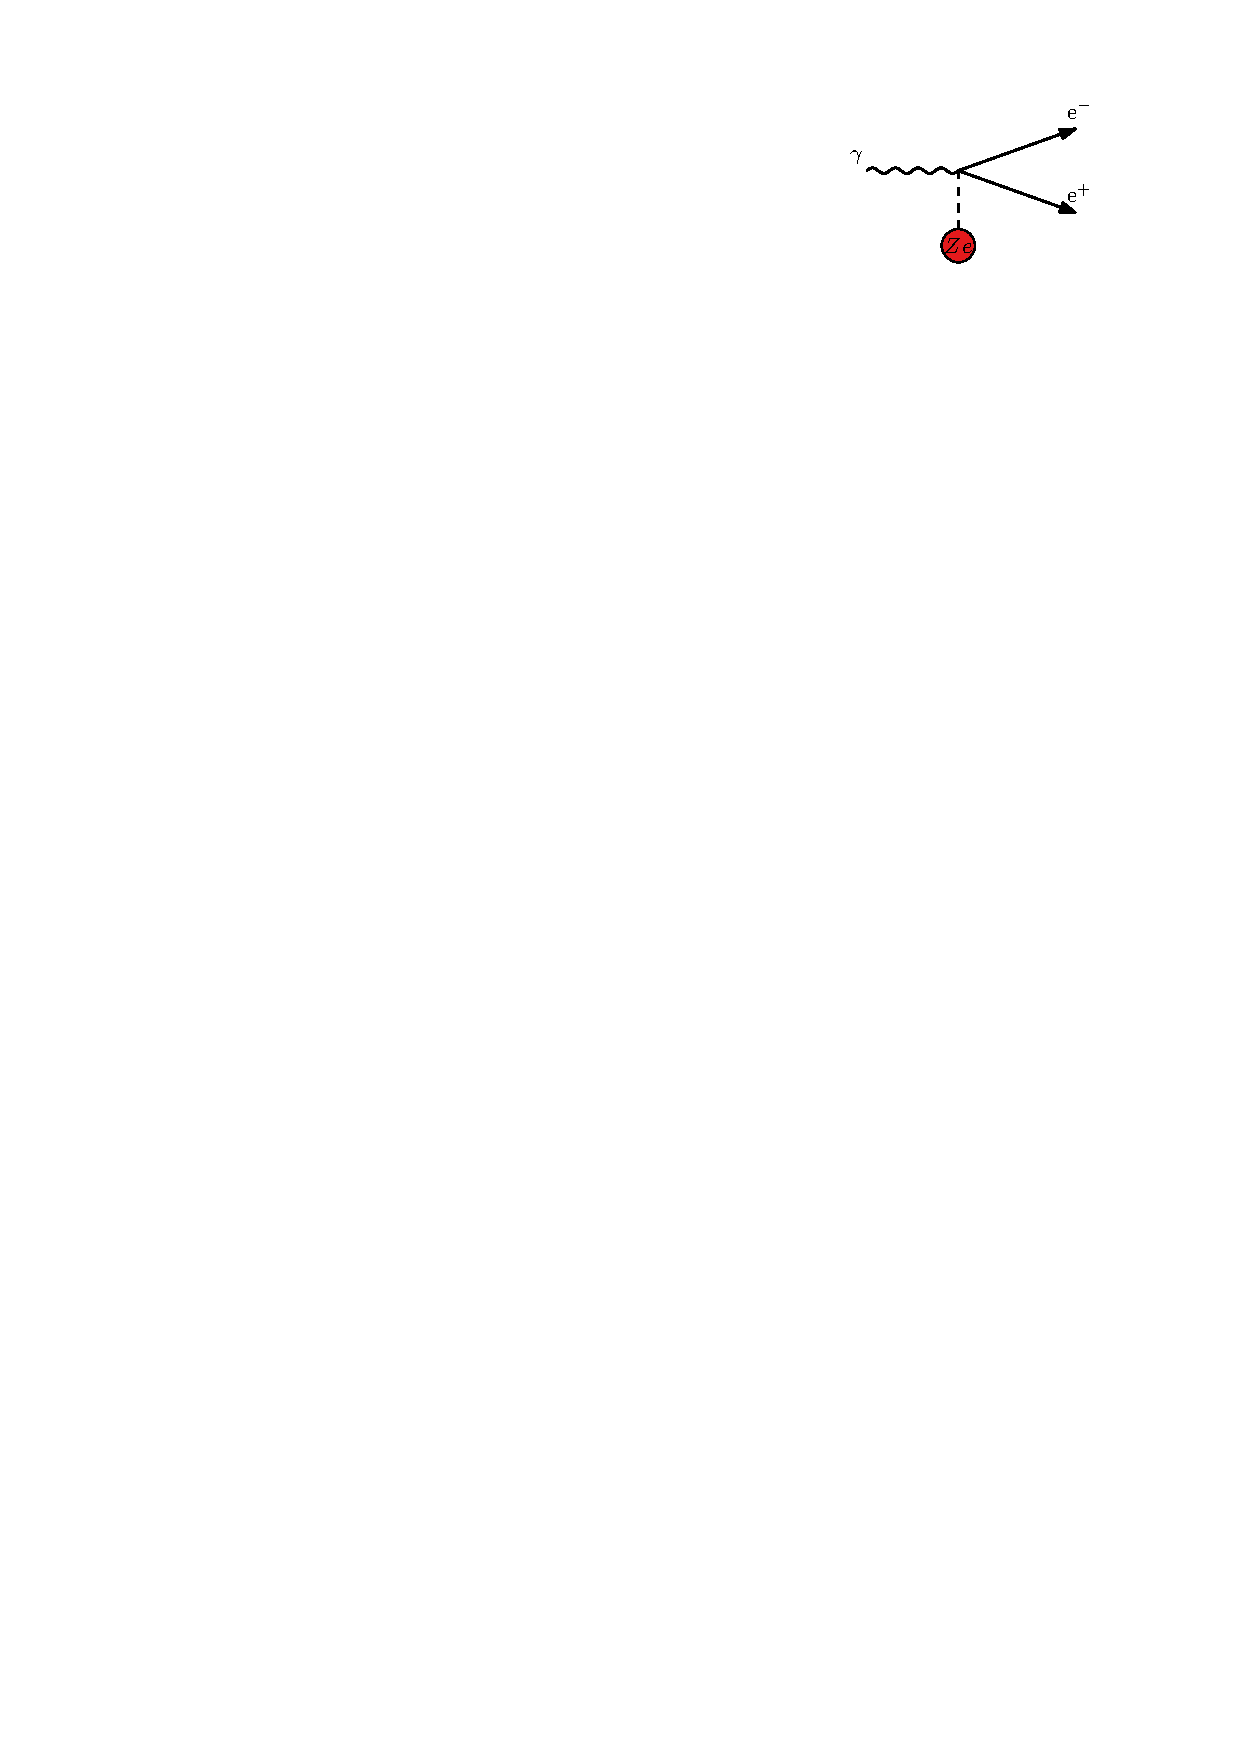
\includegraphics[width=0.8\textwidth]{./figures/pair_intro.pdf} 
				
				\vspace{0.4cm}
			\end{minipage} & $Z^2$ & $\mathrm{const}$ \\
		\end{tabular}
	\end{center}
	
\end{frame}

\begin{frame}{Interaction processes -- dependencies of the cross section}
	\centering
	\begin{overpic}[scale=0.9]{./figures/carbon.pdf}
		\put(80, -4){\footnotesize \cite{pdg}, modified}
	\end{overpic}
\end{frame}

\begin{frame}{Interaction processes -- dependencies of the cross section}
	\centering
	\begin{overpic}[scale=0.9]{./figures/lead.pdf}
		\put(80, -4){\footnotesize \cite{pdg}, modified}
	\end{overpic}
\end{frame}

\begin{frame}{Interaction processes -- material dependence}
	\centering
	\begin{overpic}[scale=0.9]{./figures/dominating_process.pdf}
		\put(80, -6){\footnotesize \cite{grupen}}
	\end{overpic}
\end{frame}

\section{Electromagnetic showers}

\begin{frame}{Electromagnetic showers}
	\begin{itemize}
		\setlength\itemsep{1.5em}
		\item interaction of high energy photons ($E_\gamma \gg 10 \, \mathrm{MeV}$) with matter
		 
		\item dominant interaction processes
		\begin{itemize}
			\item photons: pair production
			\item $\mathrm{e}^-$ / $\mathrm{e}^+$: bremsstrahlung
		\end{itemize}
		
		\item combined effect: cascade/shower of photons, electrons and positrons
		
		\item important mechanism for detecting photons in particle detectors
	\end{itemize}
\end{frame}

\note[itemize]{
	\item only a rough picture -- upcoming Calorimetry talk
	\item Picture of shower -- Blackett, Occhialini
	\item photons are uncharged and do not leave tracks in tracking detectors
}

\begin{frame}{Electromagnetic showers}
	\begin{columns}
		\column[c]{0.4\textwidth}
		\begin{itemize}
			\setlength\itemsep{1.5em}
			\item incident photon converts into $\mathrm{e}^+\mathrm{e}^-$-pair
			
			\item electrons radiate photons by bremsstrahlung
			
			\item process repeats until constituent particles reach critical energy~$E_\mathrm{c}$
			\begin{itemize}
				\item energy loss mainly due to ionization
			\end{itemize}
						
		\end{itemize}
		
		\column[c]{0.6\textwidth}
			\begin{center}
				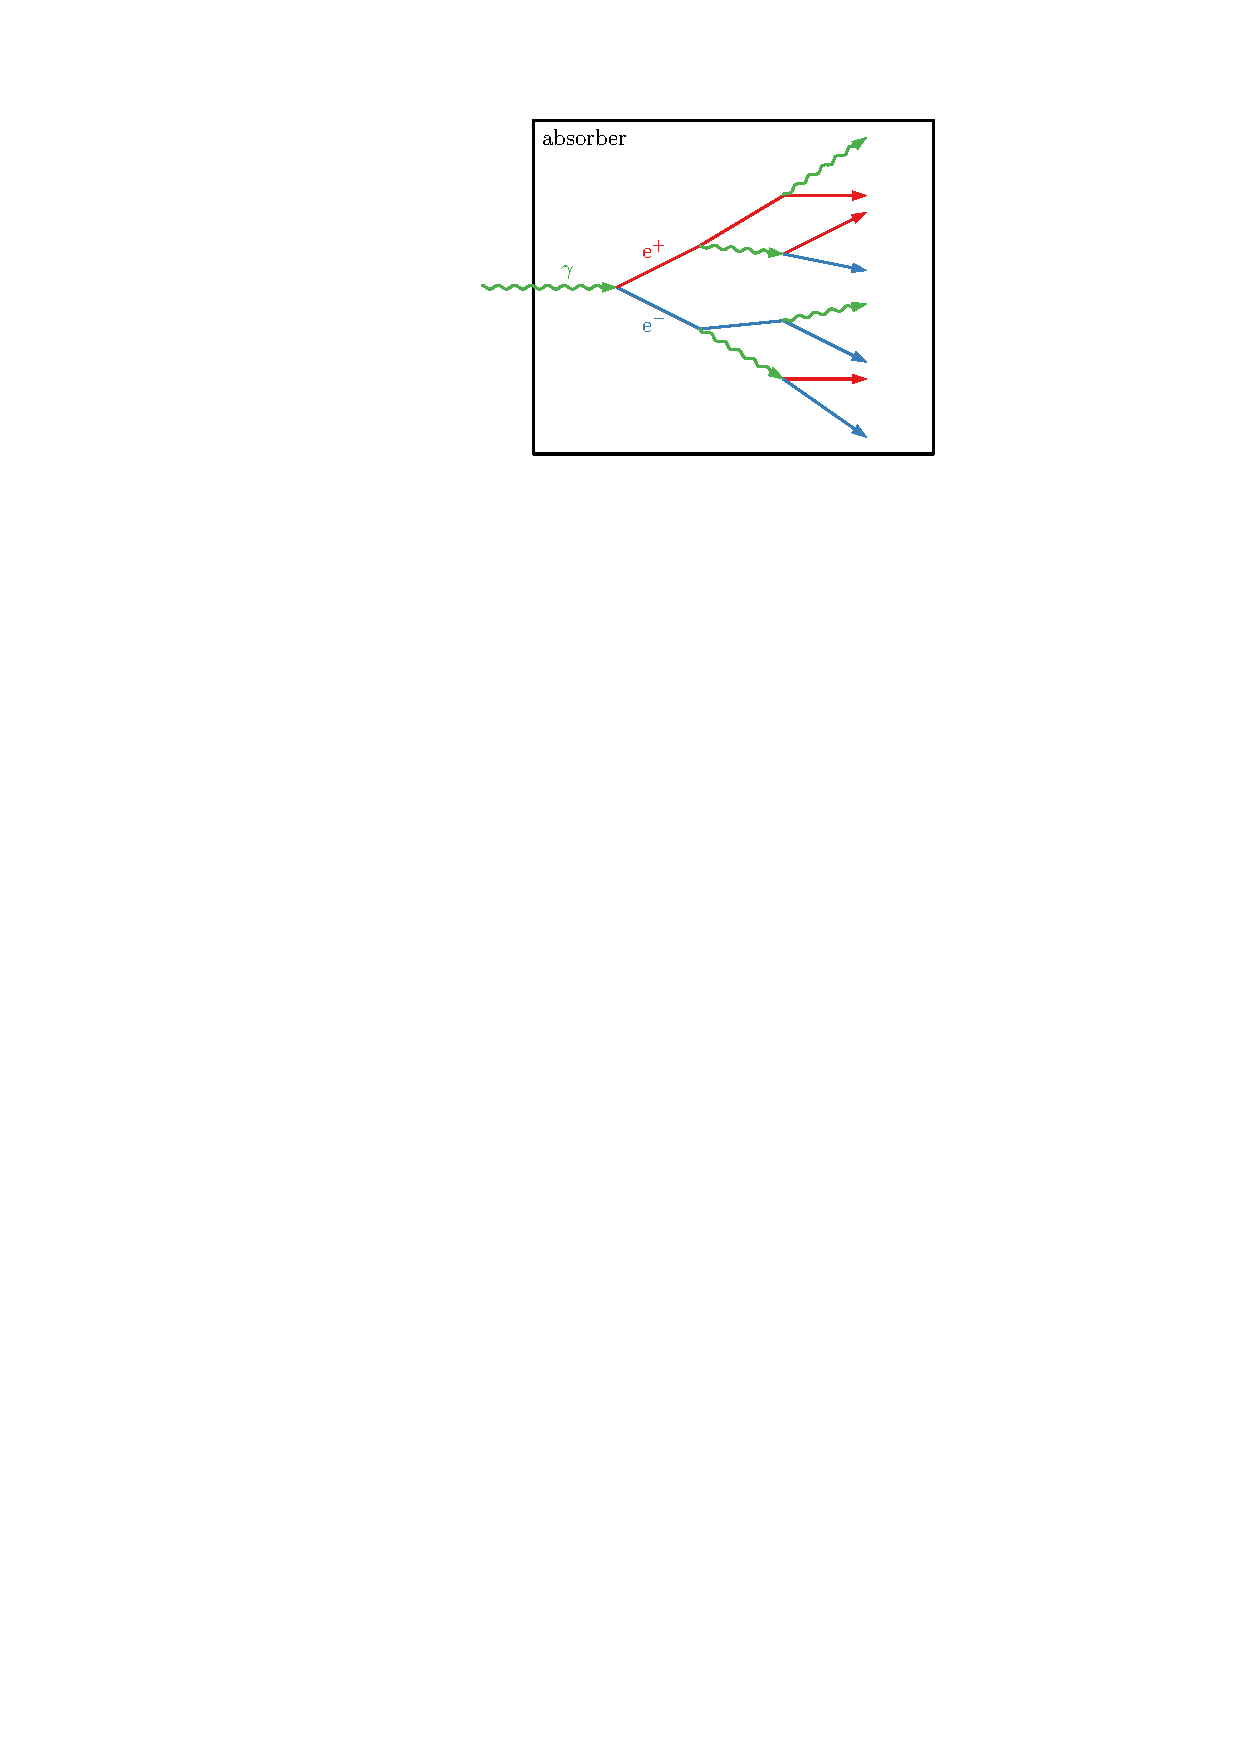
\includegraphics[width=1.0\textwidth]{./figures/shower_intro.pdf}
			\end{center}
	\end{columns}
\end{frame}

\note[itemize]{
	\item critical energy
	\begin{align*}
		\left( \frac{\mathrm{d}E(E_\mathrm{c})}{\mathrm{d}x}  \right)_\mathrm{bremss.} = \left( \frac{\mathrm{d}E(E_\mathrm{c})}{\mathrm{d}x} \right)_\mathrm{ioniz.}
	\end{align*}
}

\begin{frame}{Electromagnetic showers - Heitler's model}
	\begin{itemize}
		\setlength\itemsep{1.em}
		\item showers are a statistical process
		\begin{itemize}
			\item accurate description using Monte-Carlo methods
		\end{itemize}
		
		\item Heitler's model -- \emph{qualitative} description of a shower
	\end{itemize}
	\vfill
	Approximations:
	\begin{itemize}
		\item only pair production \& bremsstrahlung on same length scale
			\begin{align*}
				\lambda_\mathrm{pair} = \frac{9}{7} X_0 \approx X_0 \quad \rightarrow \quad \text{cascade units: } t = \frac{x}{X_0}
			\end{align*}
			
		\item 1-dimensional case: no transversal spread
		
		\item after interaction: energy evenly split between resulting particles
	\end{itemize}
\end{frame}

\note[itemize]{
	\item qualitative description -- describing only mean values
	\item also using asymptotic cross sections ($E_\gamma \rightarrow \infty$)
	\item radiation length $X_0$: electron lost $1/e$ of its energy due to bremsstrahlung
	\item assume that after $X_0$ one of the processes takes place
	
	\item 1-dim.: production of final particles in forward direction
}

\begin{frame}{Electromagnetic showers -- Heitler's model}
	\begin{center}
		\includegraphics<1>{./figures/shower_1.pdf}
		\includegraphics<2>{./figures/shower_2.pdf}
		\includegraphics<3>{./figures/shower_3.pdf}
		\includegraphics<4>{./figures/shower_4.pdf}
	\end{center}
\end{frame}

\begin{frame}{Electromagnetic showers -- Heitler's model}
	\begin{columns}
		\column[c]{0.5\textwidth}
		Quantities extracted from Heitler's model:
		\begin{itemize}
			\setlength\itemsep{1.em}
			\item number of particles at depth $t$
			\begin{align*}
				N(t) = 2^t
			\end{align*}
			
			\item energy per particle
			\begin{align*}
				E(t) = \frac{E_0}{N(t)} = E_0 \cdot 2^{-t}
			\end{align*}
			
			\item position of shower maximum $t_\mathrm{max}$ from $E(t_\mathrm{max}) = E_\mathrm{c}$
			\begin{align*}
				t_\mathrm{max} &= \log_2\left(\frac{E_0}{E_\mathrm{c}}\right)
			\end{align*}
		\end{itemize}
		
		\column[c]{0.5\textwidth}
		\begin{center}
			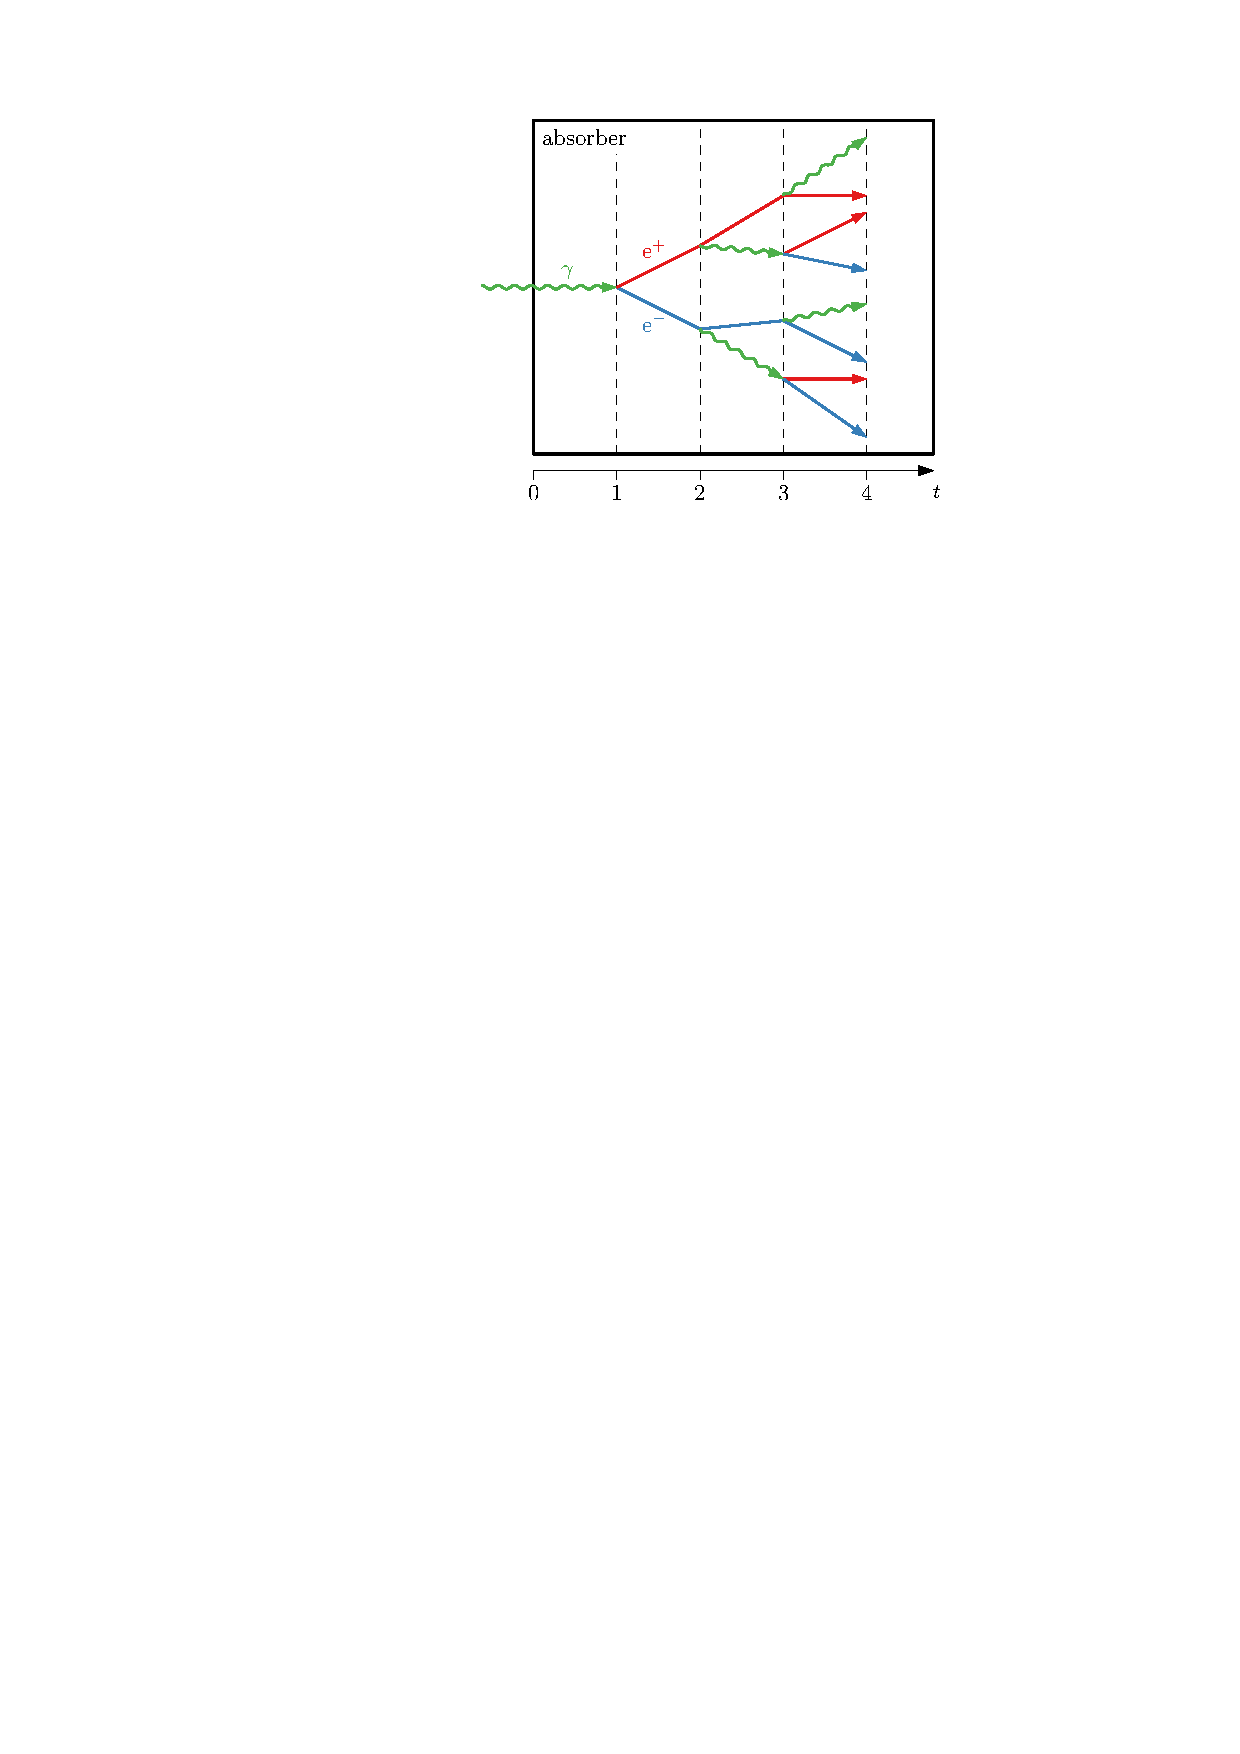
\includegraphics[width=1.0\textwidth]{./figures/shower_cascadeunits.pdf}
		\end{center}
	\end{columns}
\end{frame}

\note[itemize]{
	\item doubles with each cascade unit -- exponential increase
	
	\item energy per particle -- evenly distributed
	
	\item penetration depth -- assumption: if energy of electrons smaller than $E_\mathrm{c}$ then losses only by ionization -- cascade dies out
	
	\item from $t_\mathrm{max}$ we can also get the maximum number of particles $N_\mathrm{max} = \frac{E_0}{E_\mathrm{c}}$
	
	\item emphasize logarithmic increase of $t_\mathrm{max}$ -- nice to keep calorimeters \textit{small}
	
	\item important for energy measurement: total track length of charged particles -- proportional to energy
	\begin{align*}
		\sum_{t=0}^{t_\mathrm{max}} 2^t = 2^{t_\mathrm{max} + 1}
	\end{align*}
	
	\item $t_{95\%}$ (?)
}

\begin{frame}{Electromagnetic showers -- MC simulation}
	\begin{itemize}
		\item 95\%
	\end{itemize}
	\vfill
	Longitudinal shower profile in copper (EGS4):	
	\begin{center}
		\begin{overpic}[scale=0.8]{./figures/longitudinal_profile_edit.pdf}
			\put(70, -4){\footnotesize \cite{wigmans}, modified}
		\end{overpic}
	\end{center}
\end{frame}

\note[itemize]{
	\item Copper
}

\begin{frame}{Electromagnetic showers -- lateral spread}
	Effects causing transversal spread of the shower:
	\begin{itemize}
		\setlength\itemsep{1.5em}
		\item finite opening angles in pair production and bremsstrahlung processes
		
		\item \textbf{multiple scattering}{\tiny } of electrons and positrons in the absorber
		\begin{itemize}
			\item multiple small-angle scatterings at nuclei (TODO)
		\end{itemize}		
	\end{itemize}
	\vfill
	From Molière's theory of multiple scattering:
	\begin{itemize}
		\item $90\%$ of the energy is contained within a distance of $R_\mathrm{M}$ to the shower axis
				\begin{align*}
				R_\mathrm{M} = \frac{21\,\mathrm{MeV}}{E_\mathrm{c}} X_0
				\end{align*}
		\item e.g.\ lead $R_\mathrm{M} = 1.6 \, \mathrm{cm}$\\ $99\%$ of the shower energy is contained within $R = 3.5 \cdot R_\mathrm{M} = 5.6 \, \mathrm{cm}$
	\end{itemize}
\end{frame}

\note[itemize]{
	\item dominant process is multiple scattering
	\item independent of incident energy, since the multiple scattering is strongest for low energy particles -- only the last step is relevant for the lateral spread
	\item $99\%$ within $3.5 \, R_\mathrm{M}$
	\item lead:
	\begin{itemize}
		\item $X_0 = 0.5612 \, \mathrm{cm}$
		\item $E_\mathrm{c} = 7.43 \, \mathrm{MeV}$ for $\mathrm{e}^-$, $E_\mathrm{c} = 7.16 \, \mathrm{MeV}$ for $\mathrm{e}^+$
		\item $R_\mathrm{M} = 1.602 \, \mathrm{cm}$
	\end{itemize}
}

\begin{frame}{Electromagnetic showers -- MC simulation}
	\begin{center}
		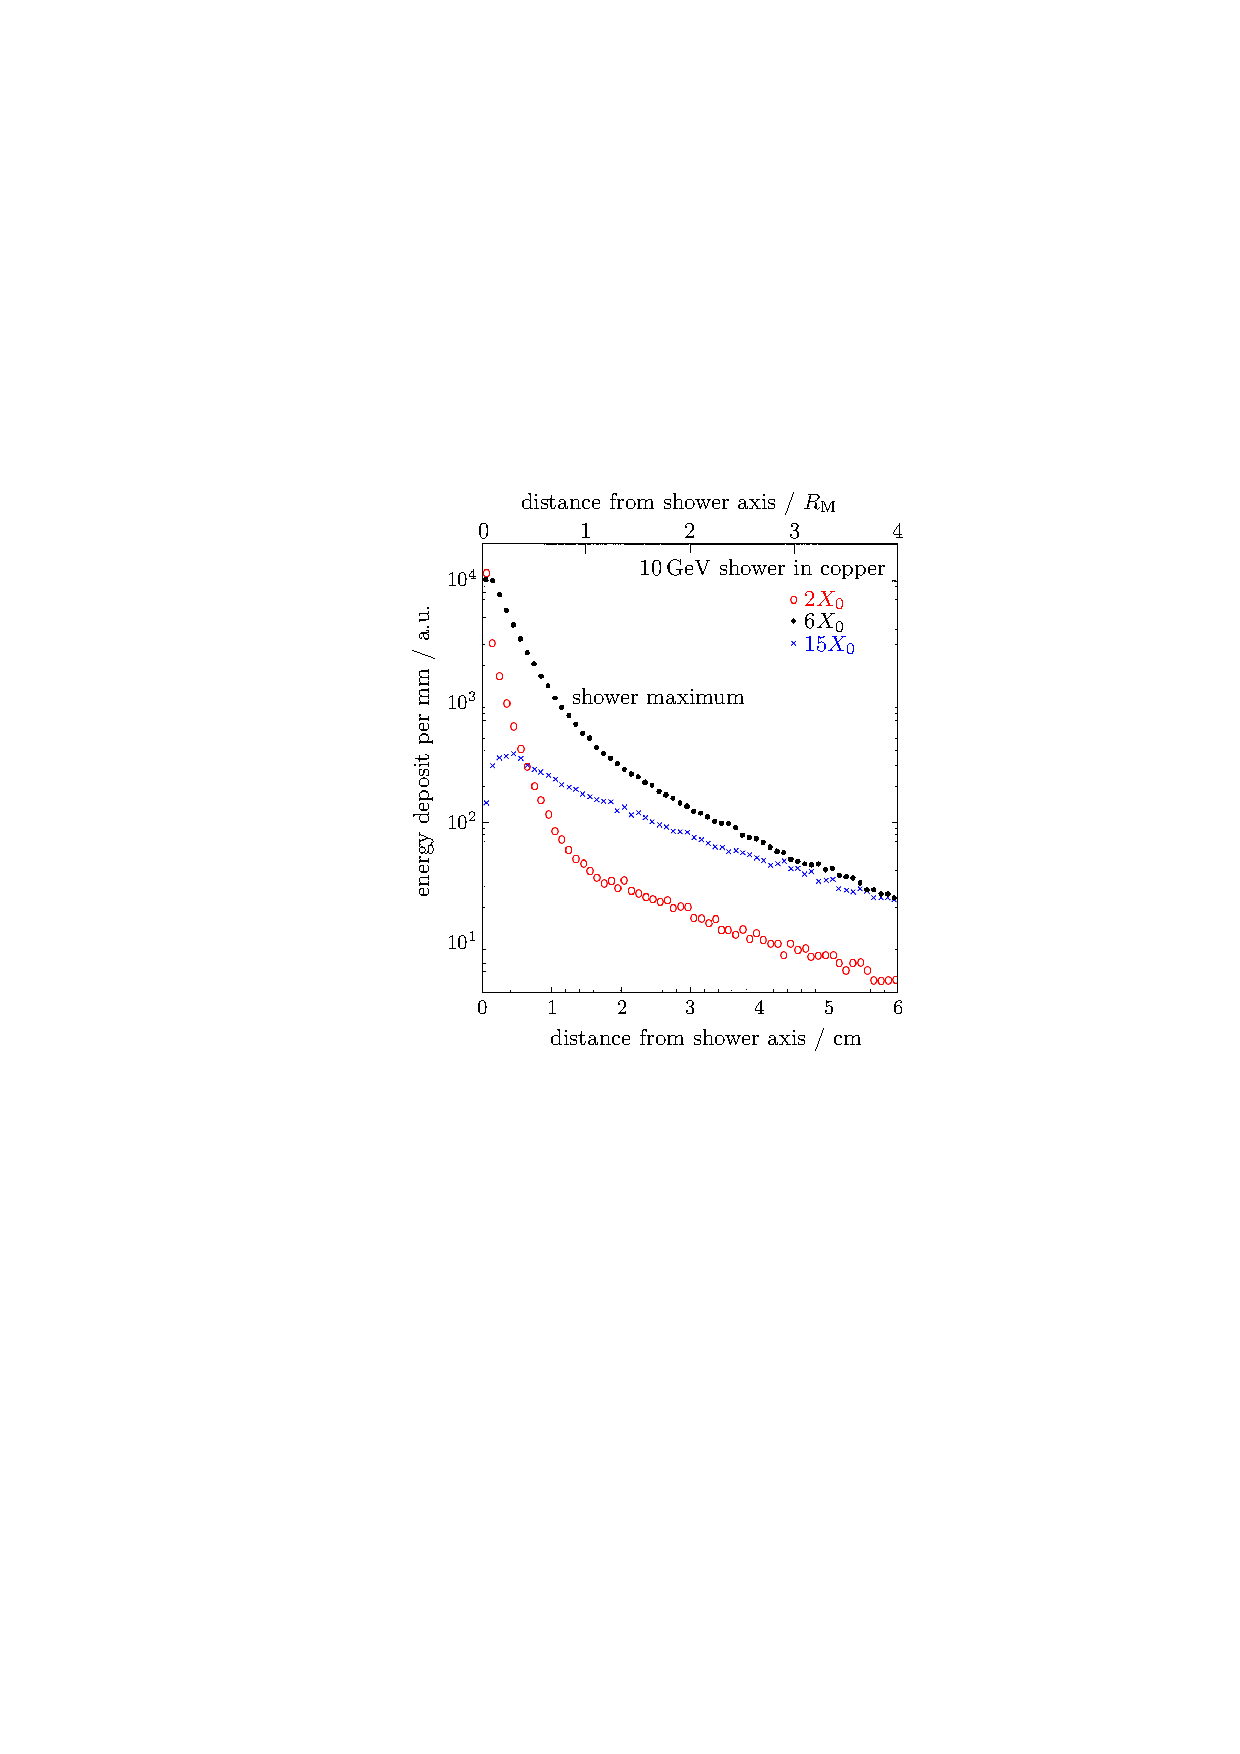
\includegraphics[scale=0.8]{./figures/transversal_profile_edit.pdf}
	\end{center}
\end{frame}

\begin{frame}{Electromagnetic showers}
	\begin{center}
		\begin{overpic}[height=0.8\textheight]{./figures/shower_brass.png}
			\put(11, -6){\footnotesize B.\ Rossi, \emph{Cosmic Rays} (1964)}
		\end{overpic}
	\end{center}
\end{frame}

\note[itemize]{
	\item $1.25 \, \mathrm{cm}$ thick brass plates
	\item placed in cloud chamber
	\item high energy electron or photon $\mathcal{O}(\mathrm{GeV})$
	
	\item air showers (?)
}



\section{Detector concepts}

\begin{frame}{Detector concepts}
	\begin{itemize}
		\item PMT (scintillation light)
		\item Photodioden (PIN, avalanche)
		\item hybrid detectors (?)
	\end{itemize}
\end{frame}

\note[itemize]{
	\item no direct detection mechanism for photons\textrightarrow charged particle interaction mandatory
}


\begin{frame}{Bibliography}
	\footnotesize
	\begin{thebibliography}{9}
		\bibitem[PDG]{pdg}
			K.A. Olive \textit{et al.} (Particle Data Group),
			\emph{The Review of Particle Physics},
			Chin.\ Phys.\ C, \textbf{38}, 090001 (2014) and 2015 update.
		
		\bibitem[Leo]{leo}
			W.\ R.\ Leo,
			\emph{Techniques for Nuclear and Particle Physics Experiments},
			Springer (1994).
		
		\bibitem[Davisson]{siegbahn}
			C.\ M.\ Davisson,
			\emph{Interaction of $\gamma$-Radiation with Matter},
			published in K.\ Siegbahn (ed.),
			\emph{Alpha- Beta- and Gamma-Ray Spectroscopy}, North-Holland Publishing Company (1979).
		
		\bibitem[Grupen, Shwarz]{grupen}
			C.\ Grupen, B.\ Shwartz,
			\emph{Particle Detectors},
			2nd edition,
			Cambridge University Press (2008).
		
		\bibitem[Heitler]{Heitler}
			W.\ Heitler,
			\emph{The Quantum Theory of Radiation},
			3rd edition, Oxford University Press (1954).
		
		\bibitem[Wigmans]{wigmans}
			R.\ Wigmans,
			\emph{Calorimetry},
			\url{http://www.roma1.infn.it/people/rahatlou/labhep/material/Wigmans_ICFA2003_Lectures.pdf} (last access: 26th April 2016).
	\end{thebibliography}
\end{frame}

\beginbackup

\begin{frame}{Gamma distribution}
	\begin{align*}
		f(x) = \frac{\beta^\alpha}{\Gamma(\alpha)} x^{\alpha - 1} e^{-\beta x}
	\end{align*}
\end{frame}

\backupend

\end{document}